%% bare_conf.tex
%% V1.4b
%% 2015/08/26
%% by Michael Shell
%% See:
%% http://www.michaelshell.org/
%% for current contact information.
%%
%% This is a skeleton file demonstrating the use of IEEEtran.cls
%% (requires IEEEtran.cls version 1.8b or later) with an IEEE
%% conference paper.
%%
%% Support sites:
%% http://www.michaelshell.org/tex/ieeetran/
%% http://www.ctan.org/pkg/ieeetran
%% and
%% http://www.ieee.org/

%%*************************************************************************
%% Legal Notice:
%% This code is offered as-is without any warranty either expressed or
%% implied; without even the implied warranty of MERCHANTABILITY or
%% FITNESS FOR A PARTICULAR PURPOSE! 
%% User assumes all risk.
%% In no event shall the IEEE or any contributor to this code be liable for
%% any damages or losses, including, but not limited to, incidental,
%% consequential, or any other damages, resulting from the use or misuse
%% of any information contained here.
%%
%% All comments are the opinions of their respective authors and are not
%% necessarily endorsed by the IEEE.
%%
%% This work is distributed under the LaTeX Project Public License (LPPL)
%% ( http://www.latex-project.org/ ) version 1.3, and may be freely used,
%% distributed and modified. A copy of the LPPL, version 1.3, is included
%% in the base LaTeX documentation of all distributions of LaTeX released
%% 2003/12/01 or later.
%% Retain all contribution notices and credits.
%% ** Modified files should be clearly indicated as such, including  **
%% ** renaming them and changing author support contact information. **
%%*************************************************************************


% *** Authors should verify (and, if needed, correct) their LaTeX system  ***
% *** with the testflow diagnostic prior to trusting their LaTeX platform ***
% *** with production work. The IEEE's font choices and paper sizes can   ***
% *** trigger bugs that do not appear when using other class files.       ***                          ***
% The testflow support page is at:
% http://www.michaelshell.org/tex/testflow/



\documentclass[conference]{IEEEtran}
% Some Computer Society conferences also require the compsoc mode option,
% but others use the standard conference format.
%
% If IEEEtran.cls has not been installed into the LaTeX system files,
% manually specify the path to it like:
% \documentclass[conference]{../sty/IEEEtran}





% Some very useful LaTeX packages include:
% (uncomment the ones you want to load)


% *** MISC UTILITY PACKAGES ***
%
%\usepackage{ifpdf}
% Heiko Oberdiek's ifpdf.sty is very useful if you need conditional
% compilation based on whether the output is pdf or dvi.
% usage:
% \ifpdf
%   % pdf code
% \else
%   % dvi code
% \fi
% The latest version of ifpdf.sty can be obtained from:
% http://www.ctan.org/pkg/ifpdf
% Also, note that IEEEtran.cls V1.7 and later provides a builtin
% \ifCLASSINFOpdf conditional that works the same way.
% When switching from latex to pdflatex and vice-versa, the compiler may
% have to be run twice to clear warning/error messages.




\usepackage{cite}
\usepackage{amsmath}
\usepackage{minted}

% *** CITATION PACKAGES ***
%
%\usepackage{cite}
% cite.sty was written by Donald Arseneau
% V1.6 and later of IEEEtran pre-defines the format of the cite.sty package
% \cite{} output to follow that of the IEEE. Loading the cite package will
% result in citation numbers being automatically sorted and properly
% "compressed/ranged". e.g., [1], [9], [2], [7], [5], [6] without using
% cite.sty will become [1], [2], [5]--[7], [9] using cite.sty. cite.sty's
% \cite will automatically add leading space, if needed. Use cite.sty's
% noadjust option (cite.sty V3.8 and later) if you want to turn this off
% such as if a citation ever needs to be enclosed in parenthesis.
% cite.sty is already installed on most LaTeX systems. Be sure and use
% version 5.0 (2009-03-20) and later if using hyperref.sty.
% The latest version can be obtained at:
% http://www.ctan.org/pkg/cite
% The documentation is contained in the cite.sty file itself.



\usepackage{mathtools}
\usepackage{fullpage,nicefrac}
\usepackage{caption}
\usepackage{subcaption}

% *** GRAPHICS RELATED PACKAGES ***
%
\ifCLASSINFOpdf
  % \usepackage[pdftex]{graphicx}
  % declare the path(s) where your graphic files are
  % \graphicspath{{../pdf/}{../jpeg/}}
  % and their extensions so you won't have to specify these with
  % every instance of \includegraphics
  % \DeclareGraphicsExtensions{.pdf,.jpeg,.png}
\else
  % or other class option (dvipsone, dvipdf, if not using dvips). graphicx
  % will default to the driver specified in the system graphics.cfg if no
  % driver is specified.
  % \usepackage[dvips]{graphicx}
  % declare the path(s) where your graphic files are
  % \graphicspath{{../eps/}}
  % and their extensions so you won't have to specify these with
  % every instance of \includegraphics
  % \DeclareGraphicsExtensions{.eps}
\fi
% graphicx was written by David Carlisle and Sebastian Rahtz. It is
% required if you want graphics, photos, etc. graphicx.sty is already
% installed on most LaTeX systems. The latest version and documentation
% can be obtained at: 
% http://www.ctan.org/pkg/graphicx
% Another good source of documentation is "Using Imported Graphics in
% LaTeX2e" by Keith Reckdahl which can be found at:
% http://www.ctan.org/pkg/epslatex
%
% latex, and pdflatex in dvi mode, support graphics in encapsulated
% postscript (.eps) format. pdflatex in pdf mode supports graphics
% in .pdf, .jpeg, .png and .mps (metapost) formats. Users should ensure
% that all non-photo figures use a vector format (.eps, .pdf, .mps) and
% not a bitmapped formats (.jpeg, .png). The IEEE frowns on bitmapped formats
% which can result in "jaggedy"/blurry rendering of lines and letters as
% well as large increases in file sizes.
%
% You can find documentation about the pdfTeX application at:
% http://www.tug.org/applications/pdftex





% *** MATH PACKAGES ***
%
%\usepackage{amsmath}
% A popular package from the American Mathematical Society that provides
% many useful and powerful commands for dealing with mathematics.
%
% Note that the amsmath package sets \interdisplaylinepenalty to 10000
% thus preventing page breaks from occurring within multiline equations. Use:
%\interdisplaylinepenalty=2500
% after loading amsmath to restore such page breaks as IEEEtran.cls normally
% does. amsmath.sty is already installed on most LaTeX systems. The latest
% version and documentation can be obtained at:
% http://www.ctan.org/pkg/amsmath

%\usepackage{appendix}
\usepackage{mathtools}
\usepackage{soul}

% *** SPECIALIZED LIST PACKAGES ***
%
%\usepackage{algorithmic}
% algorithmic.sty was written by Peter Williams and Rogerio Brito.
% This package provides an algorithmic environment fo describing algorithms.
% You can use the algorithmic environment in-text or within a figure
% environment to provide for a floating algorithm. Do NOT use the algorithm
% floating environment provided by algorithm.sty (by the same authors) or
% algorithm2e.sty (by Christophe Fiorio) as the IEEE does not use dedicated
% algorithm float types and packages that provide these will not provide
% correct IEEE style captions. The latest version and documentation of
% algorithmic.sty can be obtained at:
% http://www.ctan.org/pkg/algorithms
% Also of interest may be the (relatively newer and more customizable)
% algorithmicx.sty package by Szasz Janos:
% http://www.ctan.org/pkg/algorithmicx




% *** ALIGNMENT PACKAGES ***
%
%\usepackage{array}
% Frank Mittelbach's and David Carlisle's array.sty patches and improves
% the standard LaTeX2e array and tabular environments to provide better
% appearance and additional user controls. As the default LaTeX2e table
% generation code is lacking to the point of almost being broken with
% respect to the quality of the end results, all users are strongly
% advised to use an enhanced (at the very least that provided by array.sty)
% set of table tools. array.sty is already installed on most systems. The
% latest version and documentation can be obtained at:
% http://www.ctan.org/pkg/array


% IEEEtran contains the IEEEeqnarray family of commands that can be used to
% generate multiline equations as well as matrices, tables, etc., of high
% quality.



% *** SUBFIGURE PACKAGES ***
%\ifCLASSOPTIONcompsoc
%  \usepackage[caption=false,font=normalsize,labelfont=sf,textfont=sf]{subfig}
%\else
%  \usepackage[caption=false,font=footnotesize]{subfig}
%\fi
% subfig.sty, written by Steven Douglas Cochran, is the modern replacement
% for subfigure.sty, the latter of which is no longer maintained and is
% incompatible with some LaTeX packages including fixltx2e. However,
% subfig.sty requires and automatically loads Axel Sommerfeldt's caption.sty
% which will override IEEEtran.cls' handling of captions and this will result
% in non-IEEE style figure/table captions. To prevent this problem, be sure
% and invoke subfig.sty's "caption=false" package option (available since
% subfig.sty version 1.3, 2005/06/28) as this is will preserve IEEEtran.cls
% handling of captions.
% Note that the Computer Society format requires a larger sans serif font
% than the serif footnote size font used in traditional IEEE formatting
% and thus the need to invoke different subfig.sty package options depending
% on whether compsoc mode has been enabled.
%
% The latest version and documentation of subfig.sty can be obtained at:
% http://www.ctan.org/pkg/subfig




% *** FLOAT PACKAGES ***
%
%\usepackage{fixltx2e}
% fixltx2e, the successor to the earlier fix2col.sty, was written by
% Frank Mittelbach and David Carlisle. This package corrects a few problems
% in the LaTeX2e kernel, the most notable of which is that in current
% LaTeX2e releases, the ordering of single and double column floats is not
% guaranteed to be preserved. Thus, an unpatched LaTeX2e can allow a
% single column figure to be placed prior to an earlier double column
% figure.
% Be aware that LaTeX2e kernels dated 2015 and later have fixltx2e.sty's
% corrections already built into the system in which case a warning will
% be issued if an attempt is made to load fixltx2e.sty as it is no longer
% needed.
% The latest version and documentation can be found at:
% http://www.ctan.org/pkg/fixltx2e


%\usepackage{stfloats}
% stfloats.sty was written by Sigitas Tolusis. This package gives LaTeX2e
% the ability to do double column floats at the bottom of the page as well
% as the top. (e.g., "\begin{figure*}[!b]" is not normally possible in
% LaTeX2e). It also provides a command:
%\fnbelowfloat
% to enable the placement of footnotes below bottom floats (the standard
% LaTeX2e kernel puts them above bottom floats). This is an invasive package
% which rewrites many portions of the LaTeX2e float routines. It may not work
% with other packages that modify the LaTeX2e float routines. The latest
% version and documentation can be obtained at:
% http://www.ctan.org/pkg/stfloats
% Do not use the stfloats baselinefloat ability as the IEEE does not allow
% \baselineskip to stretch. Authors submitting work to the IEEE should note
% that the IEEE rarely uses double column equations and that authors should try
% to avoid such use. Do not be tempted to use the cuted.sty or midfloat.sty
% packages (also by Sigitas Tolusis) as the IEEE does not format its papers in
% such ways.
% Do not attempt to use stfloats with fixltx2e as they are incompatible.
% Instead, use Morten Hogholm'a dblfloatfix which combines the features
% of both fixltx2e and stfloats:
%
% \usepackage{dblfloatfix}
% The latest version can be found at:
% http://www.ctan.org/pkg/dblfloatfix




% *** PDF, URL AND HYPERLINK PACKAGES ***
%
%\usepackage{url}
% url.sty was written by Donald Arseneau. It provides better support for
% handling and breaking URLs. url.sty is already installed on most LaTeX
% systems. The latest version and documentation can be obtained at:
% http://www.ctan.org/pkg/url
% Basically, \url{my_url_here}.




% *** Do not adjust lengths that control margins, column widths, etc. ***
% *** Do not use packages that alter fonts (such as pslatex).         ***
% There should be no need to do such things with IEEEtran.cls V1.6 and later.
% (Unless specifically asked to do so by the journal or conference you plan
% to submit to, of course. )


% correct bad hyphenation here
\PassOptionsToPackage{hyphens}{url}\usepackage{hyperref}

\hyphenation{op-tical net-works semi-conduc-tor}
\DeclareMathOperator*{\argmaxA}{arg\,max}
\DeclareMathOperator*{\argminA}{arg\,min}

\usepackage{xcolor}
\usepackage{gensymb}
\newcommand{\defcommenter}[2]{%
  \expandafter\newcommand\csname #1\endcsname[1]{%
  {\color{#2}[#1: ##1]}%
  }%
}
\defcommenter{TODO}{red}
\defcommenter{JENNY}{green}
\IEEEoverridecommandlockouts
\begin{document}

%
% paper title
% Titles are generally capitalized except for words such as a, an, and, as,
% at, but, by, for, in, nor, of, on, or, the, to and up, which are usually
% not capitalized unless they are the first or last word of the title.
% Linebreaks \\ can be used within to get better formatting as desired.
% Do not put math or special symbols in the title.
\title{AutoPhase: Compiler Phase-Ordering for High-Level Synthesis 
with Deep Reinforcement Learning}
% \author{Qijing Huang*$^\dag$, Ameer Haj-Ali*$^\dag$, William Moses$^\dag$, John Xiang, Ion Stoica, Krste Asanovic, \\ John Wawrzynek \\
% \{qijing.huang, ameerh, johnxiang, istoica, krste, johnw\}@berkeley.edu, wmoses@mit.edu
% \thanks{\hspace{-0.27cm}\rule{3.15in}{0.4pt}}
% \thanks{\fontsize{9.5}{13.5}\selectfont *Equal contribution.}
% \thanks{\fontsize{9.5}{13.5}\selectfont \dag  Primary contributor.}}
\maketitle
\begin{abstract}
The performance of the code generated by a compiler depends on the order in which the optimization passes are applied.  In the context of high-level synthesis, the quality of the generated circuit relates directly to the code generated by the front-end compiler.
%The impact of compiler optimization is order-dependent.
%To produce good results, the compiler needs knowledge of the program features, the underlying systems and the run-time profiles. 
Unfortunately, choosing a good order--often referred to as the {\em phase-ordering} problem--is an NP-hard problem. As a result, existing solutions rely on a variety of sub-optimal heuristics.
%This NP-hard challenge is generally referred to as the phase-ordering challenge of the compiler.

In this paper, we evaluate a new technique to address the phase-ordering problem: deep reinforcement learning.
%The advances of deep reinforcement learning open a new horizon for addressing this challenge.
%In this paper, we explore the benefits of using deep reinforcement learning to achieve a better ordering of the compiler optimization passes.
To this end, we implement a framework that takes any group of programs and finds a sequence of passes that optimize the performance of these programs. 
%\JENNY{strictly speaking the sequence is not optimal}
% As a case study,
Without loss of generality, we instantiate this framework in the context of an LLVM compiler and target multiple High-Level Synthesis programs. 
%in theis used to target multiple High-level Synthesis programs with the LLVM compiler. 
We compare the performance of deep reinforcement learning to state-of-the-art algorithms that address the phase-ordering problem.
Overall, our framework runs one to two orders of magnitude faster than these algorithms, and achieves a 16\% improvement in circuit performance over the -O3 compiler flag.
\end{abstract}
\IEEEpeerreviewmaketitle

\section{Introduction}
High-Level Synthesis (HLS) automates the process of creating digital hardware circuits from algorithms written in high-level languages.  
Modern HLS tools~\cite{xilinx_vivado_hls,intel_hls,canis2013legup} use the same front-end as the traditional software compilers.  
They rely on traditional compiler techniques to optimize the input program's intermediate representation (IR) and produce circuits in the form of RTL code from the IRs. 
Thus, the quality of compiler front-end optimizations directly impacts the performance of HLS-generated circuit. 
Meanwhile, optimizing a program is a notoriously difficult task for the compiler. 
Programs must be in just the right form for an optimization pass to recognize it---a task which a programmer might be able to easily do, but is often difficult for the compiler.
Moreover, a programmer might have to perform different optimizations depending on the hardware platform.
Despite a decade or so of research, an expert designer can still produce RTL that outperforms the results of HLS, though it incurs huge costs both in terms of time and human capital. 
% The goal of this paper is to work towards an intelligent HLS frontend that automatically decides which  optimizations and in which order to apply. 


%The main task of a compiler is to take a program written in a high level language and produce optimized executable code to run on specific platforms. This is a notoriously difficult task. 
%To guarantee they produce correct code, compilers make conservative decisions, which can lead to missing optimizations. \JENNY{This is not the problem we try to solve as we didn't modify the passes to be more intrusive}
%Thus, despite decades of research, an expert programmer can still produce code that outperforms a compiler. Unfortunately, manually optimizing code incurs huge costs both in terms of time and human capital. 

%Compilers have been successful in accomplishing two distinct goals: they have automated many expert-programmer techniques and have allowed for programmers to write high-level and algorithmically elegant programs. However, the benefits that compilers provide do not come without cost. Programs must be in just the right form for an optimization pass to recognize it -- a task which a programmer might be able to easily do, but is often difficult for the compiler. Rather than risk producing incorrect code, the compiler must act conservatively, leading to many missed optimizations. Thus, a program manually optimized by a programmer may often outperform a program optimized by a compiler, though at a significant cost both in time and intellectual capital.


The process of HLS compilation consists of a sequence of analysis and optimization phases that are applied to the program. 
Each phase consumes the output of the previous phase, and generates a modified version of the program for the next phase. Unfortunately, these phases are not commutative which makes the order in which these phases are applied critical to the performance of the output.  
%, each of them A compiler is composed of analyses and optimizations which are simply transformations that modify programs. Unfortunately, since optimizations do not generally commute, it is crucial to apply optimizations in the proper order. 


Consider the program in Figure \ref{fig:norm1}, which normalizes a vector. Without any optimizations the \verb|norm| function will take $\Theta(n^2)$ to normalize a vector. However, a smart compiler will implement the \textit{loop invariant code motion (LICM)}\cite[Sec.~13.2]{Muchnick97} optimization, which allows it to move the call to \verb|mag| above the loop, resulting in the code on the left column in Figure \ref{fig:norm2}. This brings the runtime down to $\Theta(n)$ -- a big speedup improvement. Another optimization the compiler could perform is \textit{(function) inlining}\cite[Sec.~15.2]{Muchnick97}. With inlining, a call to a function is simply replaced with the body of the function, reducing the overhead of the function call. Applying inlining to the code 
%in Figure \ref{fig:norm2}, 
will result in the code in the right column of Figure~\ref{fig:norm2}.
\begin{figure}[h]
     \centering
         \centering
\begin{minted}[fontsize=\footnotesize]{c}
__attribute__((const))
double mag(const double *A, int n) {
    double sum = 0;
    for(int i=0; i<n; i++){
        sum += A[i] * A[i];
    }
    return sqrt(sum);
}
void norm(double *restrict out,
          const double *restrict in, int n) {
    for(int i=0; i<n; i++) {
        out[i] = in[i] / mag(in, n);
    }
}
\end{minted}
\vspace*{-0.2cm}
\caption{A simple program to normalize a vector. \vspace*{-0.1cm}}
    \label{fig:norm1}
\end{figure}
\begin{figure*}[h]
     \centering
     \begin{subfigure}[b]{0.46\textwidth}
         \centering
\begin{minted}[fontsize=\footnotesize]{c}
void norm(double *restrict out,
          const double *restrict in, int n) {
    double precompute = mag(in, n);
    for(int i=0; i<n; i++) {
        out[i] = in[i] / precompute;
    }
}
\end{minted}
    %\label{fig:norm2}
\end{subfigure}
     \hfill
     \begin{subfigure}[b]{0.46\textwidth}
         \centering
\begin{minted}[fontsize=\footnotesize]{c}
void norm(double *restrict out,
          const double *restrict in, int n) {
    double precompute, sum = 0;
    for(int i=0; i<n; i++){
        sum += A[i] * A[i];
    }
    precompute = sqrt(sum);
    for(int i=0; i<n; i++) {
        out[i] = in[i] / precompute;
    }
}
\end{minted}
     \end{subfigure}
     \vspace{-0.2cm}
     \caption{Progressively applying LICM (left) then inlining (right) to the code in Figure~\ref{fig:norm1}.}
    \label{fig:norm2}
    \vspace{-0.4cm}
\end{figure*}
\begin{figure*}[!h]
     \centering
     \begin{subfigure}[b]{0.46\textwidth}
         \centering
\begin{minted}[fontsize=\footnotesize]{c}
void norm(double *restrict out,
          const double *restrict in, int n) {
    for(int i=0; i<n; i++) {
        double sum = 0;
        for(int j=0; j<n; j++){
            sum += A[j] * A[j];
        }
        out[i] = in[i] / sqrt(sum);
    }
}
\end{minted}
    %\label{fig:norm4}
\end{subfigure}
     \hfill
     \begin{subfigure}[b]{0.46\textwidth}
         \centering
\begin{minted}[fontsize=\footnotesize]{c}
void norm(double *restrict out,
          const double *restrict in, int n) {
    double sum;
    for(int i=0; i<n; i++) {
        sum = 0;
        for(int j=0; j<n; j++){
            sum += A[j] * A[j];
        }
        out[i] = in[i] / sqrt(sum);
    }
}
\end{minted}
     \end{subfigure}
          \vspace{-0.3cm}
     \caption{Progressively applying inlining (left) then LICM (right) to the code in Figure~\ref{fig:norm1}.}
     \label{fig:norm3}
     \vspace{-0.5cm}
\end{figure*}



Consider applying these optimization passes in the opposite order: first inlining then LICM. After inlining, we get the code on the left of Figure~\ref{fig:norm3}. Once again we get a modest speedup, having eliminated $n$ function calls, though our runtime is still $\Theta(n^2)$. If the compiler afterwards attempted to apply LICM, we would find the code on the right of Figure~\ref{fig:norm3}. LICM was able to successfully move the allocation of sum outside the loop. However, it was unable to move the instruction setting \verb|sum=0| outside the loop, as doing so would mean that all iterations excluding the first would have a garbage value for sum. Thus, the internal loop could not be moved out.

Consequently, having the wrong phase ordering for a program can mean the difference between one's program running in $\Theta(n^2)$ versus $\Theta(n)$. It is thus crucial to determine the optimal phase ordering for the program for it to run efficiently. Unfortunately, not only is this a difficult task, but the optimal phase ordering may vary from program to program.
The goal of this paper is to provide a mechanism for automatically determining good phase orderings for HLS programs to optimize for the circuit speed. 
%targeting hardware designs.

Recent advancements in deep reinforcement learning (RL)~\cite{sutton1998} offer opportunities to address the phase ordering challenge. 
In deep RL algorithms, software agents take actions in an environment to optimize accumulative rewards. 
%Generally, deep RL algorithms interact with the environment and are rewarded based on their actions. 
Based on these rewards and environment observations, statistical machine learning is applied to estimate the long-term benefit of the actions and optimize these actions accordingly. 
%In this work, we explore the benefits of applying deep RL algorithms to improve the quality of results (QoR) of HLS. 
Significant challenges exist in understanding how to formulate the phase ordering optimization problem in an RL framework. 
In this paper, we investigate two techniques to characterize the optimization state.
One is to directly use salient features from the program.
The other one is to use the applied optimizations as features without any information from the programs. 
We implement a framework that takes a group of programs and quickly finds a phase ordering that produces better quality of results.
Our main contributions are:
\begin{itemize}
    %\item Modified the LLVM compiler to extract 
    %program features that describe the program structure.  %describe the number of different operations from a specific HLS program.
    \item An analysis of two methods to represent program state in the RL setting: (1) program features and (2) a histogram of previously applied passes. We conclude why the later approach is more efficient in achieving better algorithm optimization time and circuit cycle count.
    \item A framework that integrates the compiler with the deep RL algorithms. This framework takes a group of programs as an input and robustly generates the optimal sequence of passes to apply. 
    %\item A study of our approach in multiple RL settings with significant performance and runtime improvements versus state-of-the-art approaches for compiler optimization.
    \item An evaluation and comparison of multiple RL algorithms against state-of-the-art approaches for compiler phase-ordering showing that RL runs one to two orders of magnitude faster and achieves $16\%$ better performance over -O3.
\end{itemize}

%The rest of the paper is organized a follows. Section~\ref{sec:bg} gives a brief background on compiler optimization, RL and related works. In Sections \ref{sec:framework} and \ref{sec:DRLA} the implemented framework and the deep RL architecture implementation are described, respectively. The framework is evaluated in Section~\ref{sec:results}, compared to state-of-the-art approaches for compiler optimization and a thorough analysis is presented. The paper is concluded in Section~\ref{sec:conc}.
\section{background} % 1.5 pages
\label{sec:bg}
%\subsection{Compiler Optimization}
%Compilers often package groups of optimizations into ``optimization levels'' -O0 (no optimization), -O1 (some optimization) –O2 (more optimization), -O3 (most optimization) for ease. 
%While these optimization levels offer a simple set of choices for developers, they are somewhat arbitrarily chosen by compiler-designers and often most benefit the runtime of certain benchmark programs. 
%Often, -O3 will produce worse\TODO{Ameer: Jenny, why worse?} performance than -O2 on the same program. 
%While these optimization levels offer a simple set of choices for developers, they are handpicked by the compiler-designers and often benefit certain groups of benchmark programs. 
%The compiler community has attempted to address the issue by selecting a particular set of compiler optimization passes on a per-program or per-target basis for software\TODO{Ameer: no mention of hardware and focus on software}
%\JENNY{This is sw only as there is not much work on HLS, for hw it is mention in the related works}, with a few highly-cited examples \cite{triantafyllis2003compiler,almagor2004finding,pan2006fast}.

\subsection{Compiler Phase-ordering}
Compilers execute optimization passes to transform programs into more efficient forms to run on various hardware targets.
Groups of optimizations are often packaged into ``optimization levels'' -O0 (no optimization), -O1 (some optimization) –O2 (more optimization), -O3 (most optimization) for ease. 
While these optimization levels offer a simple set of choices for developers, they are handpicked by the compiler-designers and often most benefit certain groups of benchmark programs. 
The compiler community has attempted to address the issue by selecting a particular set of compiler optimizations on a per-program or per-target basis for software\cite{triantafyllis2003compiler,almagor2004finding,pan2006fast}.


Since the search space of phase-ordering is too large for exhaustive search, many heuristics have been proposed to explore the space by using machine learning. 
Huang~\textit{et al.} tried to address this challenge for HLS applications by using modified greedy algorithms~\cite{huang2013effect}\cite{huang2015effect}. %It achieved 16\% improvement vs -O3 on HLS generated circuits.  %to apply a new optimization to an existing sequence and keep the best one or three sequences at each 
In~\cite{agakov2006using} both independent and Markov models were applied to automatically target an optimized search space for iterative methods to improve the search results.
In~\cite{2003Stephenson}, genetic algorithms were used to tune heuristic priority functions for three compiler optimization passes. 
Milepost\cite{fursin2011milepost} used machine learning to determine the set of passes to apply to a given program, based on a static analysis of its features. It achieved 11\% execution time improvement over -O3, for the ARC reconfigurable processor on the MiBench program suite1.
In~\cite{2012Kulkarni} the challenge was formulated as a Markov process and supervised learning was used to predict the next optimization, based on the current program state.
Wang \textit{et al.}~\cite{wang2018}, described a relationship between machine learning and compiler optimization, where the program features are used as an observation, without explicitly providing results. In this work, we tried using the program features as an observation but found that it faces several challenges explained in Section~\ref{sec:DRLA}.
\subsection{Reinforcement Learning}

Reinforcement learning (RL) is a machine learning approach in which an agent continually interacts with the environment~\cite{kaelbling1996reinforcement}. In particular, the agent observes the state of the environment, and based on this observation takes an action. The goal of the RL agent is then to compute a policy--a mapping between the environment states and actions--that maximizes a long term reward. 
%by taking actions. These actions are generally the output of a policy that takes as an input a state/observation. The objective of RL is to find a policy that maximizes the reward an agent receives while interacting with the environment.

RL can be viewed as a stochastic optimization solution for solving Markov Decision Processes (MDPs)~\cite{bellman1957}, when the MDP is not known. An MDP 
%models the system with an agent that wants to optimize a given objective (such as the score in a game) by making a sequence of decisions. Given the current state, a decision is made, which leads to a new state. More formally, the Markov decision process 
is defined by a tuple with four elements:
${S,A,P(s,a),r(s,a)}$ where $S$ is the set of states of the environment, $A$ describes the set of actions or transitions between states, $s' {\raise.17ex\hbox{$\scriptstyle\mathtt{\sim}$}}
 P(s,a)$ describes the probability distribution of next states given the current state and action and $r(s,a):S \times A \rightarrow R$ is the reward of taking action $a$ in state $s$. Given an MDP, the goal of the agent is to gain the largest possible aggregate reward. The objective of an RL algorithm associated with an MDP is to find a decision policy $\pi^*:s\rightarrow A$ that achieves this goal for that MDP:
 %, by mapping states to actions, that maximize the reward:
\begin{multline}
\label{eq:MDP}
    \pi^* = \argmaxA_\pi E_{\tau{\raise.05ex\hbox{$\scriptstyle\mathtt{\sim}$}}\rho_{\pi(\tau)}} \left[\sum_{t}^{}r(s_t,a_t) \right] = \\
    \argmaxA_\pi \sum_{t=1}^{T}E_{(s_t,a_t){\raise.05ex\hbox{$\scriptstyle\mathtt{\sim}$}}\rho_{\pi(s_t,a_t)}}\left[r(s_t,a_t)\right].
\end{multline}

Deep RL leverages a neural network to learn the policy (and sometimes the reward function). Recently, Deep RL has achieved impressive results, such as learning to play 49 Atari games with human-level capabilities~\cite{mnih2015}, and defeating the Go world champion~\cite{silver2016}. Over the past couple of years, a plethora of deep RL techniques have been proposed~\cite{mnih2016,ross2011,sutton2000,watkins1992q}. In this paper, we focus on two algorithms: Policy Gradient (PG)~\cite{sutton2000} and Deep Q-Network (DQN), commonly referred to as Q-Learning~\cite{watkins1992q}. We chose these algorithms as they are simple, mature, and adequate to solve the problem. 

PG computes the policy directly by differentiating the aggregate reward \textit{i.e.}, the term in Equation~\ref{eq:MDP}:
\begin{multline}
\label{eq:policygradient}
    \nabla_\theta J =  \nabla_\theta E_{\tau{\raise.05ex\hbox{$\scriptstyle\mathtt{\sim}$}}\rho_{\pi(\tau)}} \left[\sum_{t}^{}r(s_t,a_t) \right] = \\
    E_{\tau{\raise.05ex\hbox{$\scriptstyle\mathtt{\sim}$}}\rho_{\pi(\tau)}} \left[(\sum_{t}^{}\nabla_\theta log\pi_\theta(a_t|s_t))(\sum_{t}^{}r(s_t,a_t))\right] \approx \\
    \frac{1}{N}\sum_{i=1}^{N} \left[ (\sum_{t}^{}\nabla_\theta log\pi_\theta(a_{i,t}|s_{i,t}))(\sum_{t}^{}r(s_{i,t},a_{i,t})) \right]
\end{multline}
and then updating the network parameters (weights) in the direction of the gradient:
\begin{equation}
    \theta \leftarrow \theta+\alpha\nabla_\theta J,
\end{equation}
where $\alpha$ is called the learning rate. PG is an on-policy method in that it uses only the current policy to compute the new policy.

In contrast, DQN is an off-policy method which takes partially random actions to explore the state space. The DQN's goal is to find which actions will maximize future rewards from a given state. To do so DQN computes a $Q$-function, $Q(s_i, a_i)$ that predicts the future overall reward of taking action $a_i$ from state $s_i$. To compute this $Q$-function, DQN uses a neural network paramterized by weights $\phi$). More formally:

\begin{equation}
\label{eq:Dqn}
    y_i = r(s_i,a_i) + \argmaxA_{a'_i}Q_\phi(s'_i,a'_i)\\
\end{equation}
\begin{equation}
    \phi \leftarrow \argminA_{\phi}\sum_i||Q_\phi(s_i,a_i)-y_i||^2,
\end{equation}
\noindent
where $y_i$ is the target result, $a_i$ and $s_i$ are the current action and state respectively, $a'_i$ and $s'_i$ are the next action and state respectively, and $r(s_i,a_i)$ is the reward for taking action $a_i$ at state $s_i$. On top of that, the policy is basically defined as follow:
\begin{equation}
    \pi_\theta(a_t|s_t) =
    \begin{cases}
    1 & \text{if } a_t =\argmaxA_{a_t}Q_\phi(s'_t,a'_t)\\
    0              & \text{otherwise}
\end{cases}
\end{equation}

\section{Simulation Framework} 
\label{sec:framework}
We leverage an existing open-source HLS framework called LegUp \cite{canis2013legup} that takes a C program as input and outputs a hardware RTL design. 
In \cite{huang2013effect}, an approach is devised to quickly determine the number of hardware execution cycles without requiring time-consuming logic simulation.
We develop our reinforcement learning simulator environment based on the existing harness provided by LegUp and  validate our final results by going through the time-consuming logic simulation. The framework takes a program (or multiple programs) and intelligently explores the space of possible passes to figure out an optimal pass sequence to apply. The framework is illustrated in Figure~\ref{fig:framework}.

\subsection{HLS Compiler}
Our framework takes a set of programs as input and compiles them using the Clang front-end of the LLVM compiler. LLVM represents programs in a hardware-independent intermediate representation (IR). Optimization and analysis passes act as transformations on the IR, taking a program as input and emitting a new IR as output. The HLS tool LegUp is invoked after the compiler optimization as a back-end pass, which transforms LLVM IR into hardware modules.
%The compute logic is turned into a hardware datapath and the control logic is turned into a hardware FSM respectively by the HLS tool. 
%Its SDC-based scheduler \cite{cong2006efficient} operates at the basic block level to exploit the instruction-level parallelism. 

\subsection{Clock-cycle Time Profiler}
Once the hardware RTL is generated one could run a hardware simulation to gather the cycle count results of the synthesized circuit. This process is quite time-consuming, hindering RL and all other optimization approaches. Therefore, we approximate cycle count using the profiler in LegUp~\cite{huang2013effect}, which runs $20\times$ faster than hardware simulation. 
In LegUp, the frequency of the generated circuits is set as a compiler constraint that directs the HLS scheduling algorithm. In other words, HLS tool will always try to generate hardware that can run at a certain frequency. In our experiment setting, without loss of generality, we set the target frequency of all generated hardware to 50MHz.
%The profiler first runs the software program to gather information on the number of times each basic block is executed, then multiplies it with the clock cycle time of the basic block determined by the HLS scheduler to produce the total clock cycle time of the circuit. This software approach is $20\times$ faster than hardware simulation, which significantly reduces the runtime bottleneck of the deep reinforcement learning algorithm. 

\subsection{IR Feature Extractor}
In addition to the LegUp backend tools, we developed analysis passes to extract 56 static features from the program, such as the number of basic blocks, branches, and instructions of various types. 
%Each individual feature is insufficient to guide the machine learning algorithm.
We use these features as partially observable states for the RL learning and hope the neural network can capture the correlation of certain combination of these features and certain optimization. Unfortunately, due to the page limit, we could not include the table of features. 
%All the features we gather are listed in Table~\ref{tab:tab1} in the appendix. 
%The framework takes a program or multiple ones and compiles them using the LLVM compiler, which was modified to output the program features. The HLS toolchain is used to extract the number of cycles that are used as the cost function to the RL architecture to find the optimal passes. 

\subsection{Deep Reinforcement Learning Framework}
We wrapped compilation utilities into a Python script and wrote an environment simulator with APIs similar to an OpenAI gym~\cite{brockman2016openai}. Our utilities take an input a program (as LLVM IR) and returns the program feature vectors and the total number of clock cycles. We consider two types of features as the state for the RL: the current program IR and the sequence of passes that have been applied. The overall flow works as follows:
\begin{enumerate}
\item The program is compiled into LLVM IR. 
\item LegUp compiles the LLVM IR into hardware RTL and produces an estimated clock-cycle time for the generated circuit. 
\item The IR feature extractor is run to extract program features. 
\item The clock-cycle time and program features are fed into various machine learning algorithms (random, genetic, greedy, and RL) to derive a good LLVM optimization sequence. In RL specifically, the clock-cycle time is used for reward calculation, and the program features are used as partially observable states for the RL agents. 
\item In iterative methods (\textit{i.e.}, greedy algorithm, genetic algorithm, and RL), the algorithm then predicts the next best action to take. In RL, the action would be the next optimization to apply to the end of an existing sequence of passes. In a modified greedy algorithm, the next action could be the next best place to insert the optimization pass.
\item New LLVM IR is generated after the new optimization sequence is applied. 
\item The machine learning algorithm iterates through steps 2)--6) until convergence.
\end{enumerate}


\begin{figure}[h!]
    \centering
    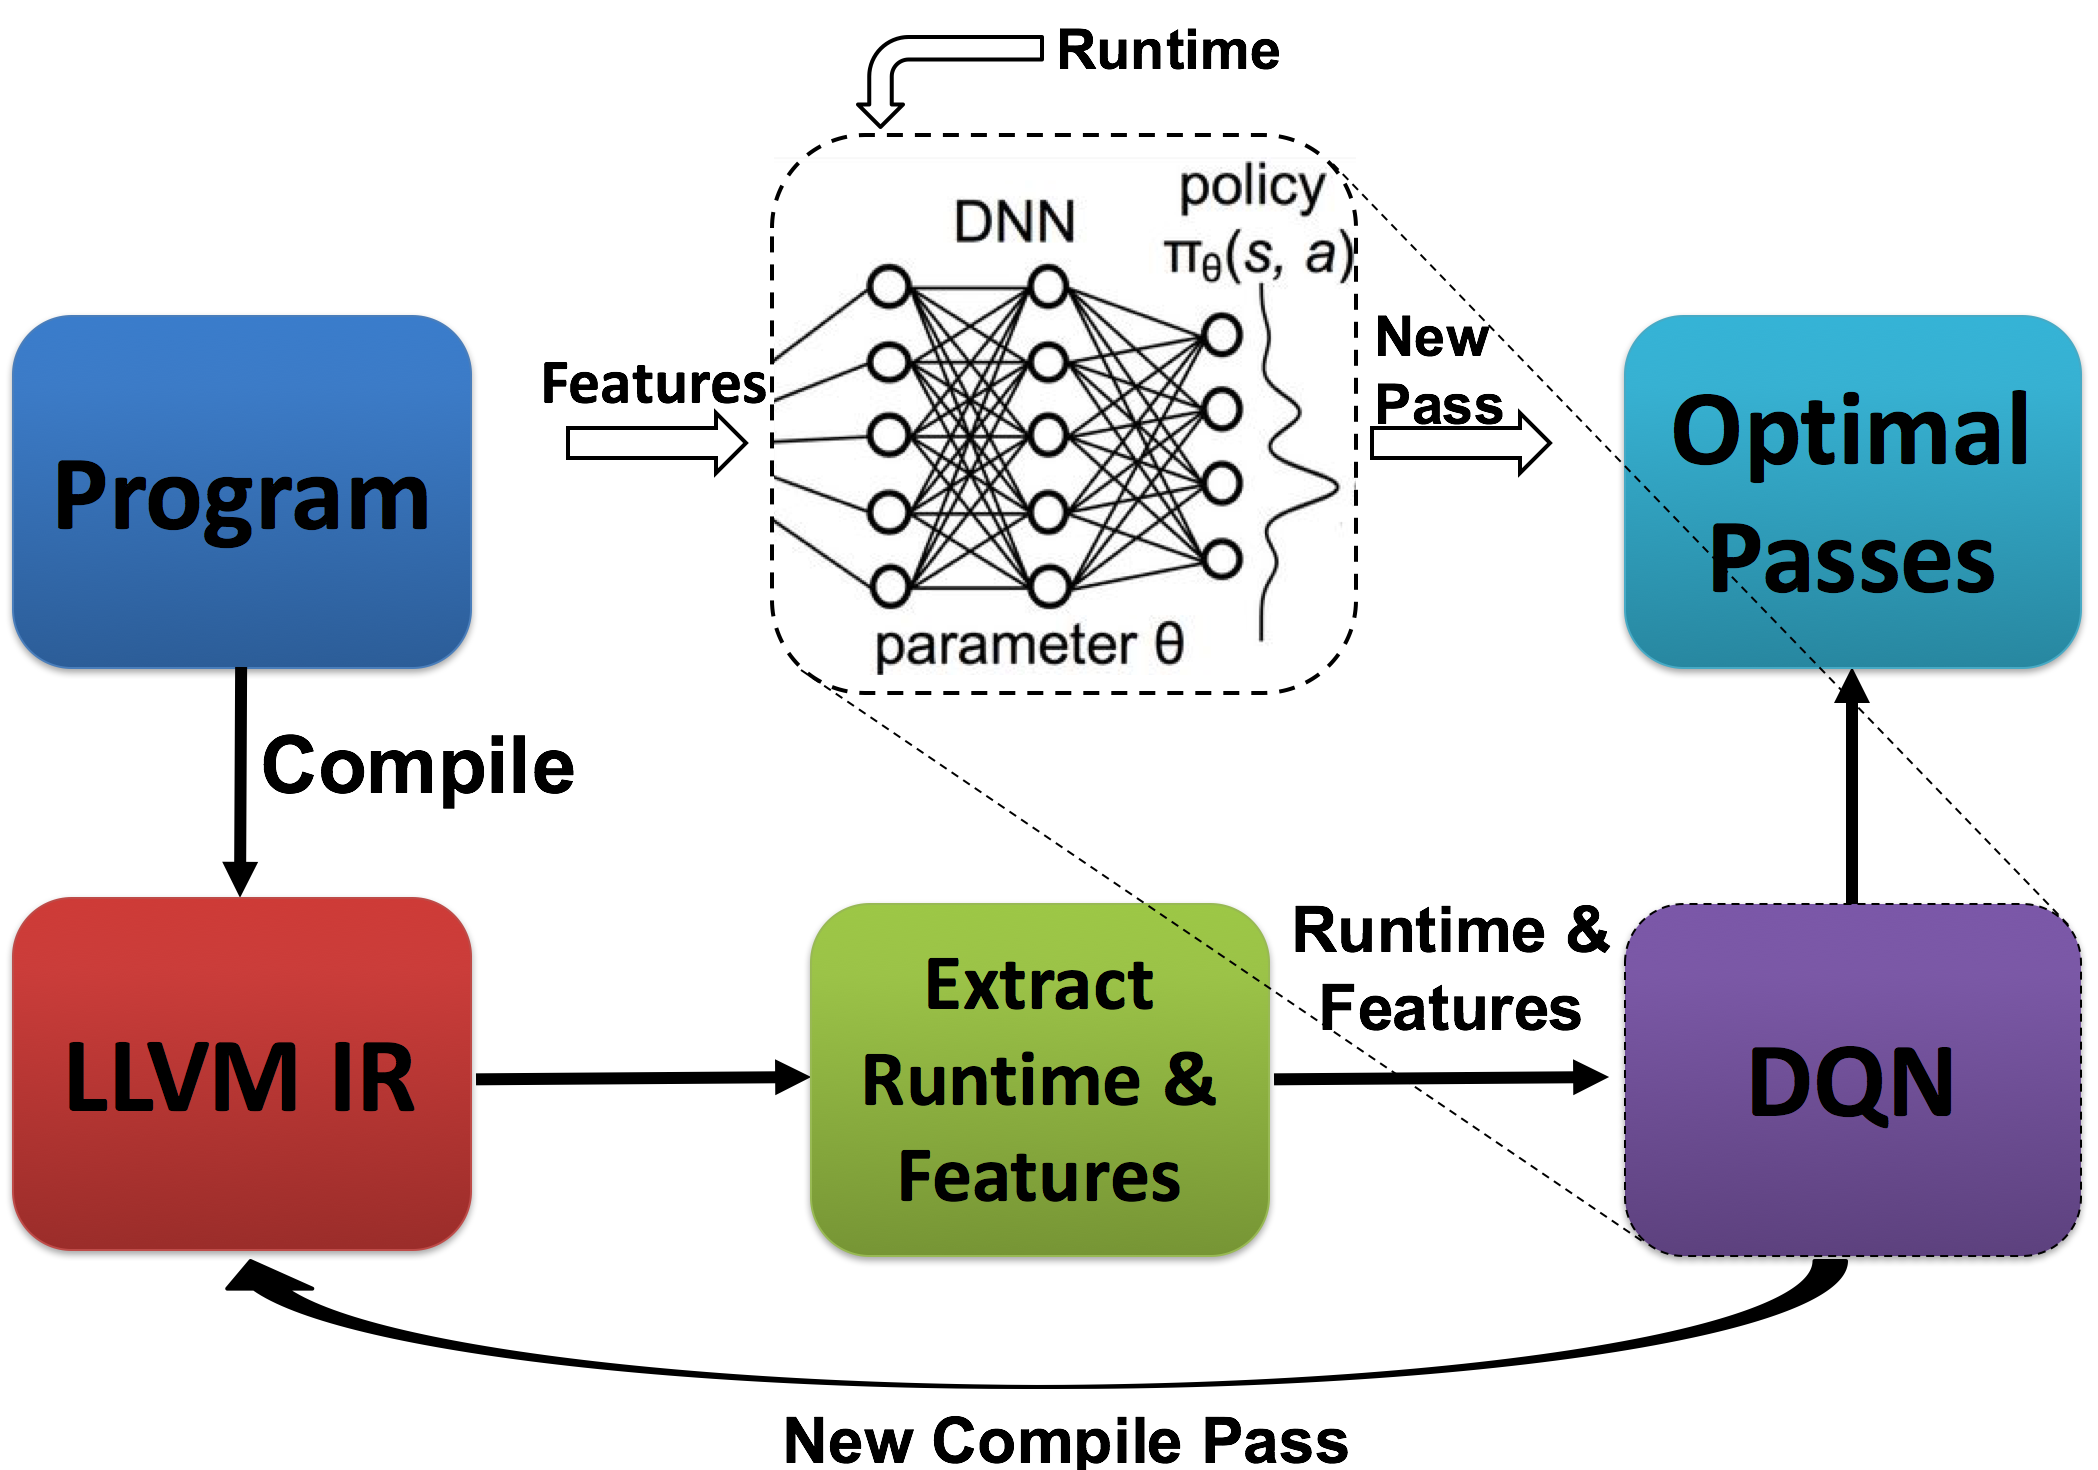
\includegraphics[width=0.5\textwidth]{Figures/framework.png}
    \caption{A block diagram of our framework. The programs are compiled using the Clang/LLVM, features and cycles are extracted from the IR and HLS toolchain respectively, and are afterwards fed to the RL network that tries to learn the optimal passes.  \vspace*{-0.5cm}}
    \label{fig:framework}
\end{figure}

\section{Deep Reinforcement Learning Architecture} % 1 page 
\label{sec:DRLA}
DQN and PG are used in the implemented architecture.
DQN can take advantage of optimal substructures during training. It can also alleviate the impact of long compilation (environment step) time by greatly reducing the data needed. Wang \textit{et al.}~\cite{wang2018} proposed to convert a program into an observation by extracting all the features of the program, \textit{i.e.} number of every operation. Similarly, we extracted program features from the programs. %as listed in Table \ref{tab:tab1}\JENNY{TODO include appendix or not?}\TODO{Ameer: I think so} in the appendix.

Another approach is to use the actions (passes) themselves as observations. In other words, the input of the network (observation) was defined as a histogram of the passes given so far and the passes were given an index from zero to the number of passes. The output is the next pass to apply. This allows the network to keep track of passes applied so far and learn which sequences should be applied to maximize the reward.

We also considered various initial transformations on the programs before running a learning algorithm. We added seven prepasses that will invoke necessary program analysis passes for all programs. This approach reduces the difficulty for the network in finding the best initialization passes. The reward was defined as the negative number of cycles, and thus a higher reward means a lower number of cycles to run the program.

\subsection{Program Features Versus Histogram of Actions}
To evaluate the two approaches, we ran the framework on 12 HLS benchmarks. We trained each benchmark for $30$ minutes. The methodology is described in Section~\ref{sec:results}. Figure~\ref{fig:model-action} shows the circuit speedup as function of time for the two approaches with DQN as the RL algorithm, and -O3, normalized to the performance without any optimization. Both approaches achieve similar performance. The average performance improvement is $13.3\%$ over -O3 and $50\%$ over the performance without any optimization. These improvements are mainly due to the fact that DQN efficiently and robustly learns which passes are useful and which are not.

Figure~\ref{fig:gsm_model_action} shows the mean cycles as a function of time when running the framework on one of the programs (gsm) using the two approaches. Both approaches improve the program's mean cycles over time. We observe two things: (1) Rather than having a smooth line, the instability and chaotic behavior of DQN is seen in the jumps of mean cycles of both approaches. (2) The DQN approach that uses previous passes as the input observation is more stable than using the program features.

\begin{figure}[!t]
    \centering        
    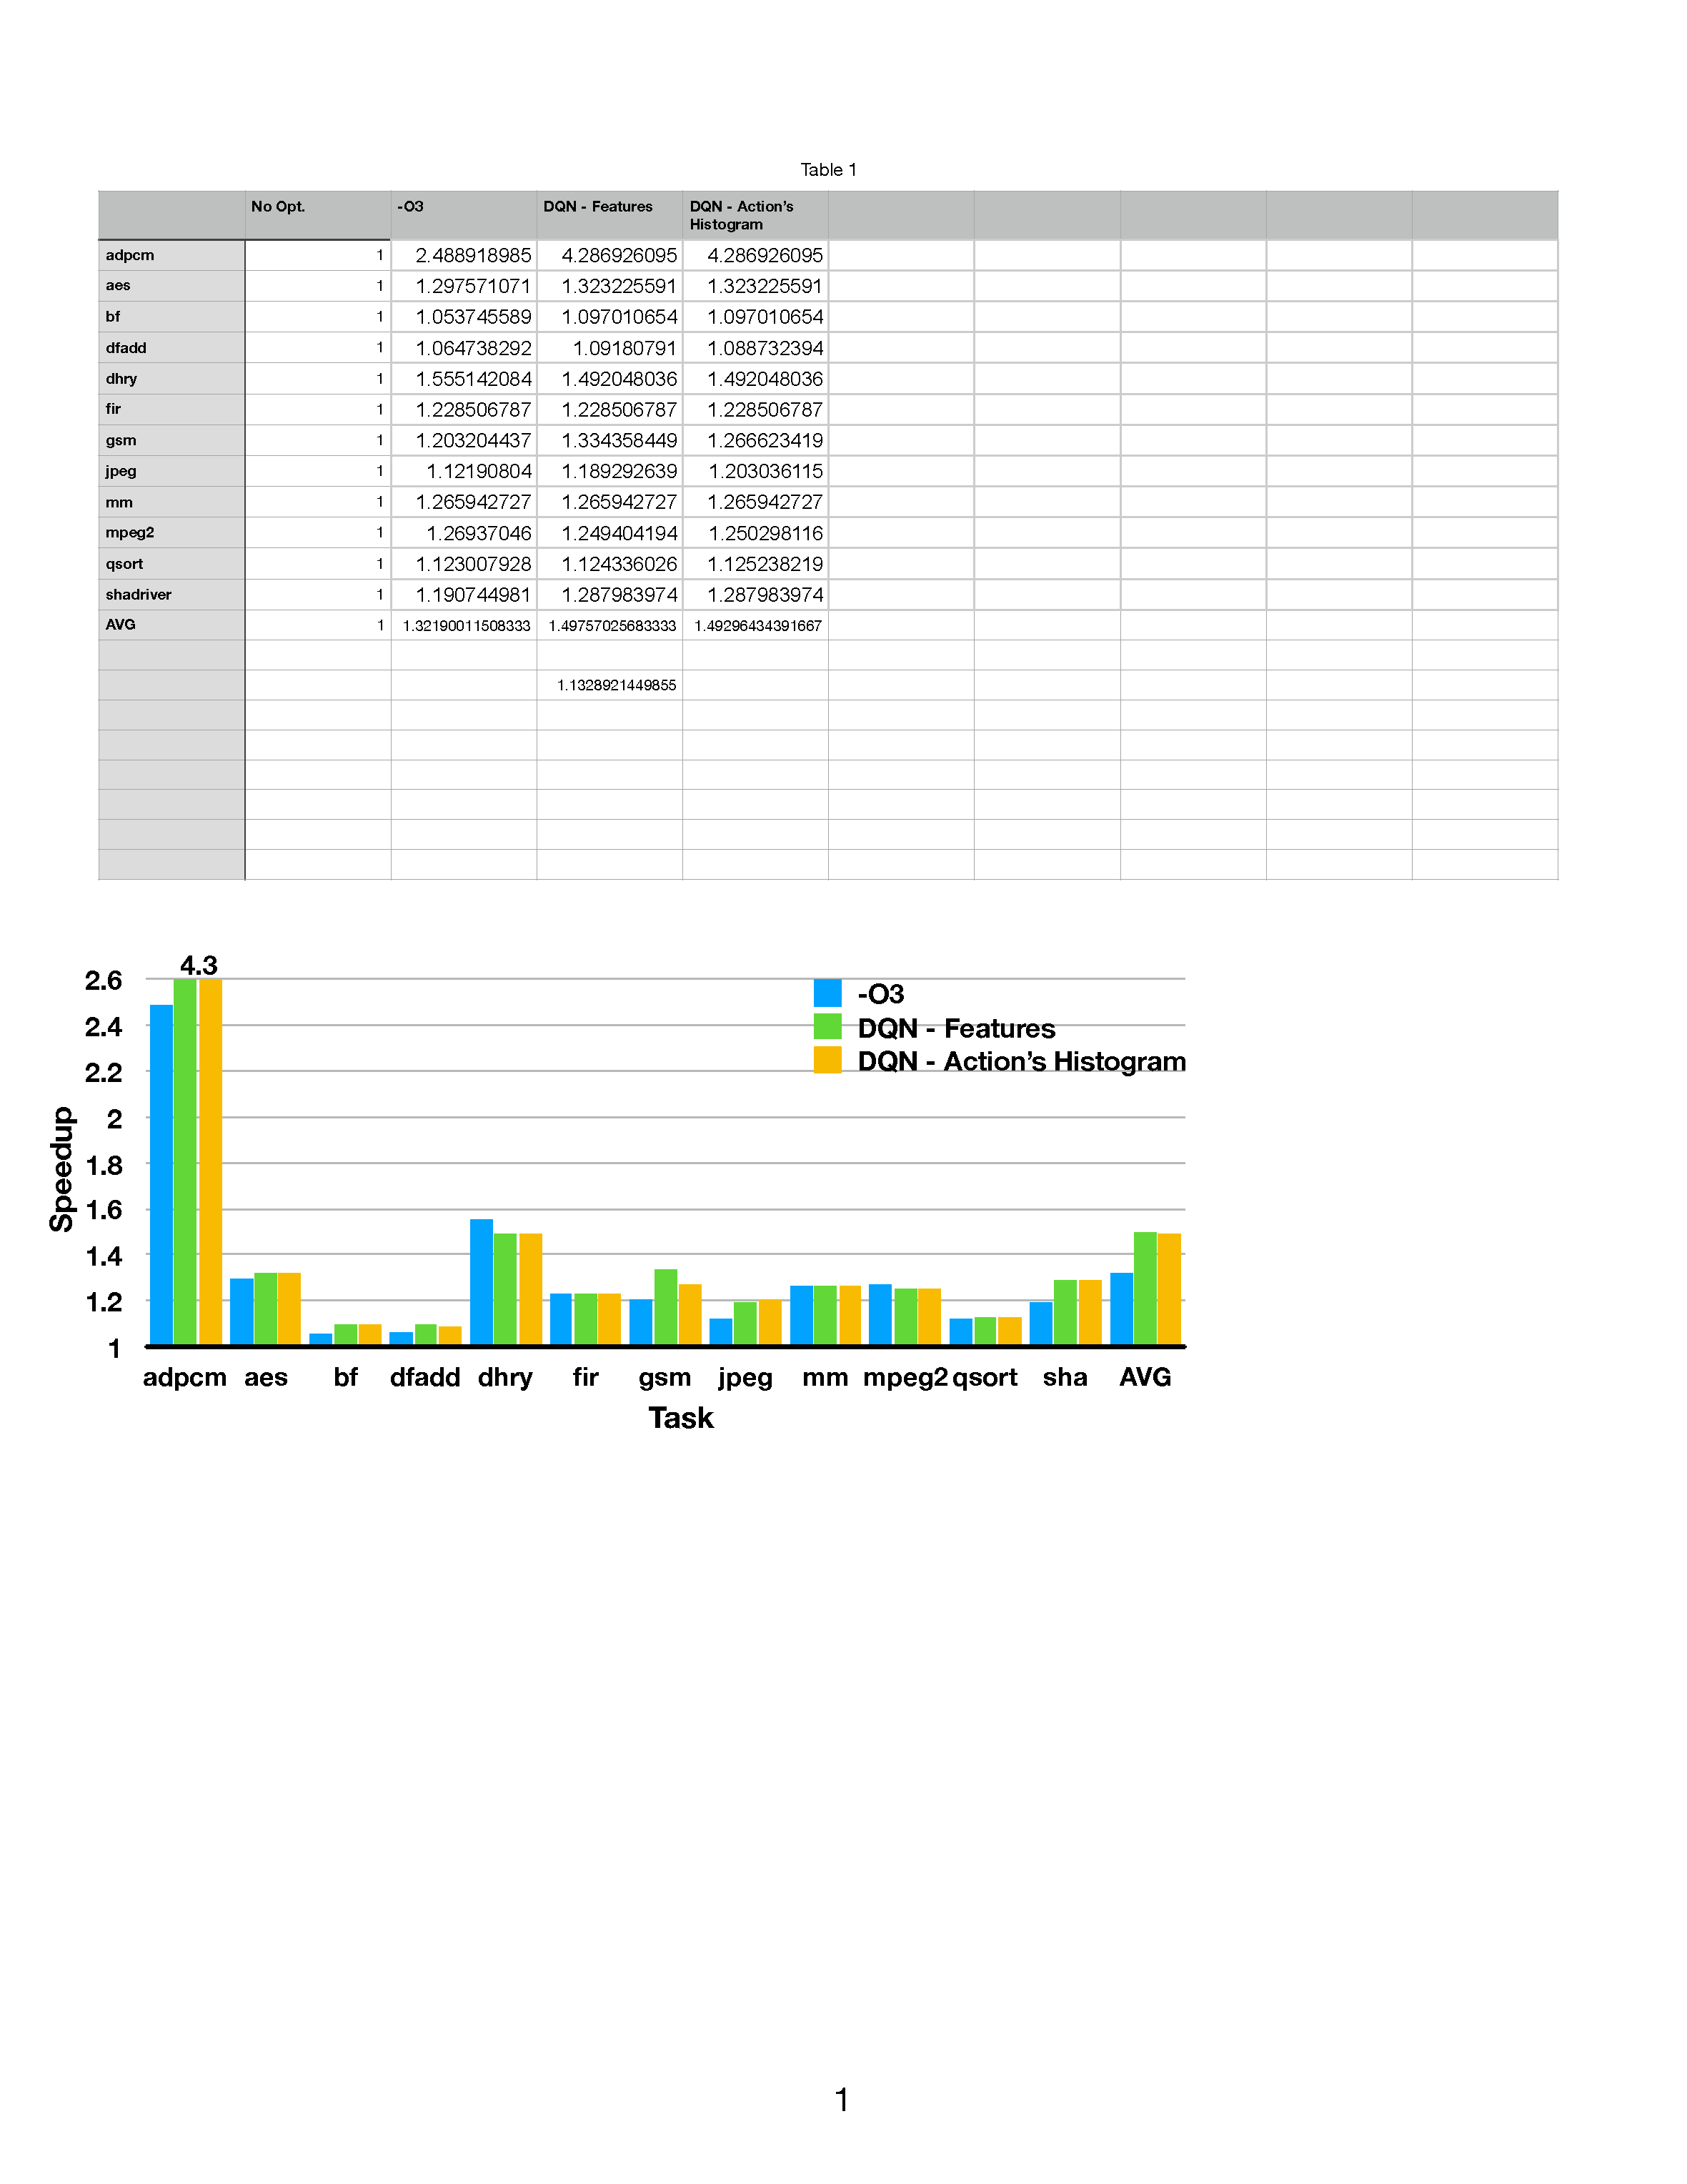
\includegraphics[trim={1.1cm 17.7cm 11.5cm 21.5cm},clip,width=0.5\textwidth]{Figures/model-action2.pdf} 
    \caption{The circuit speedup as function of algorithm training time for different optimization algorithms normalized to the performance without any optimization. The RL framework ran for 30 minutes on each program. \vspace*{-0.6cm}}
    \label{fig:model-action}
\end{figure}
\begin{figure}[!t]
    \centering
    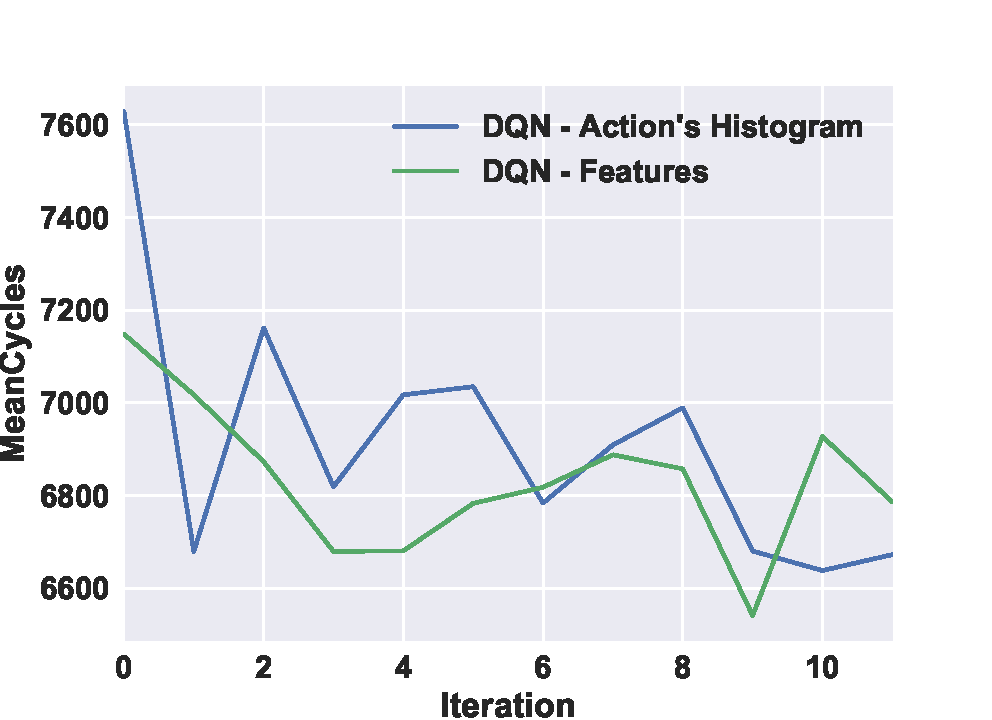
\includegraphics[trim={0cm 0cm 0cm 1cm},clip,width=0.5\textwidth]{Figures/gsm_model_action2.pdf}
    \vspace{-0.5cm}
    \caption{The mean cycles as function of time when running the framework on the gsm task. \vspace*{-0.6cm}}
    \label{fig:gsm_model_action}
\end{figure}

While both program feature and histogram approaches are efficient for operating on a single program, the histogram approach provided better performance in the long run. We observed that several passes are effective only if preceded by other passes, which may not change the program features significantly. For example, a pass may change only the order of instructions, but not their distribution. The network mistakenly learns to apply these effective passes directly and gain a zero benefit, resulting in unstable behavior. Furthermore, the space of features for various programs is sufficiently complex that it is difficult for a simple framework to learn, and it is not possible to derive a perfect optimization ordering on multiple programs simultaneously since each program has different features.

In contrast, using previous actions as the observation guarantees that after applying each pass the observation changes, making it less ambiguous for the network to learn. In addition, it enables operating on multiple programs simultaneously since the observation is independent from the program, which provides faster training. To further optimize the time it takes to run the framework we could also leverage the fact that the observations are directly extracted from the actions. This makes it possible to roll out an entire trajectory of actions and observations from the policy without compiling the programs. Effectively, we apply a pass, generate the new histogram, feed the new histogram to the policy again, which outputs a new pass and so on. The only things missing in this technique are the intermediate rewards that could be calculated by compiling the program after applying each pass, which we are trying to avoid as it takes a long time. 

In PG, the term in Equation~\ref{eq:policygradient} that depends on the reward value is the sum of rewards in the entire trajectory. This value could be obtained directly by compiling the program once at the end with all the applied passes. This makes using PG feasible although it generally requires more data samples and time to learn compared to DQN. In addition, in DQN, we could %compile once and average the reward for the labels in Equation~\ref{eq:Dqn} or 
compile a few times, each one after applying a sequence of actions and average the reward for all these actions. Beyond significantly reducing the training time, this approach helps alleviate the sparsity of rewards in cases where multiple passes are necessary to get a single reward and make the seemingly ineffective passes more effective. 


To operate on multiple programs simultaneously, the reward function was defined as follows:
\begin{multline}
     -reward_t = \sqrt[\leftroot{-2}\uproot{2}n]{C\_Prog_1(t) \cdot ... \cdot C\_Prog_n(t)} -
    \\
    \sqrt[\leftroot{-2}\uproot{2}n]{C\_Prog_1(t-1) \cdot ... \cdot C\_Prog_n(t-1)},
\end{multline}
where $n$ is the number of programs and $C\_Prog_i(t)$ is the cycle count of program $i$ at time step $t$. This reward function was chosen to guarantee that all programs are equally optimized; any improvement in one will positively affect the reward and make the rewards more dense. To speed the training process we took a multithreaded approach inspired by~\cite{mnih2016}. We implemented a multithreaded program that compiles the different programs simultaneously taking the same actions (passes) in each program.


%Note that the DQN and PG versions used in this work are in their simplest form and there are many improvements that mainly aim to reduce variance~\cite{van2016,Baxter2001}. Since our ultimate goal is to find a single trajectory that achieves the maximum reward and given that we want to find it as fast as possible, we can tradeoff this variance. %The performance of DQN could also be improved by using Double DQN (DDQN)~\cite{van2016}, which was used in the implemented framework.


 
% The most straightforward way to convert a program into an observation is achieved by extracting all the features of the program, \textit{i.e.} number of every operation as proposed by Wang \textit{et al.}~\cite{wang2018}. The features we extracted from the compiled programs are listed in Table \ref{tab:tab1} in the appendix. Nevertheless, these features proved to be not useful even after rigorous efforts on multiple RL algorithms, network configurations, which include fully connected (FC) networks, recurrent neural network~\cite{HausknechtS2015drl} and numerous network parameters search. We observed that several effective passes are effective only if preceded by other passes, which unfortunately do not change the observation. For example, if the pass only changes the order of instructions but not their distribution. The network mistakenly learns to apply these effective passes directly and gain a zero reward. %The issue is illustrated in Figure~\ref{fig:problem1}. 
% Furthermore, the space of features for various programs is too large and complicated to learn in a simple framework and it is not possible to learn on multiple programs simultaneously since each program has different features.
% \begin{figure}
%     \centering
%     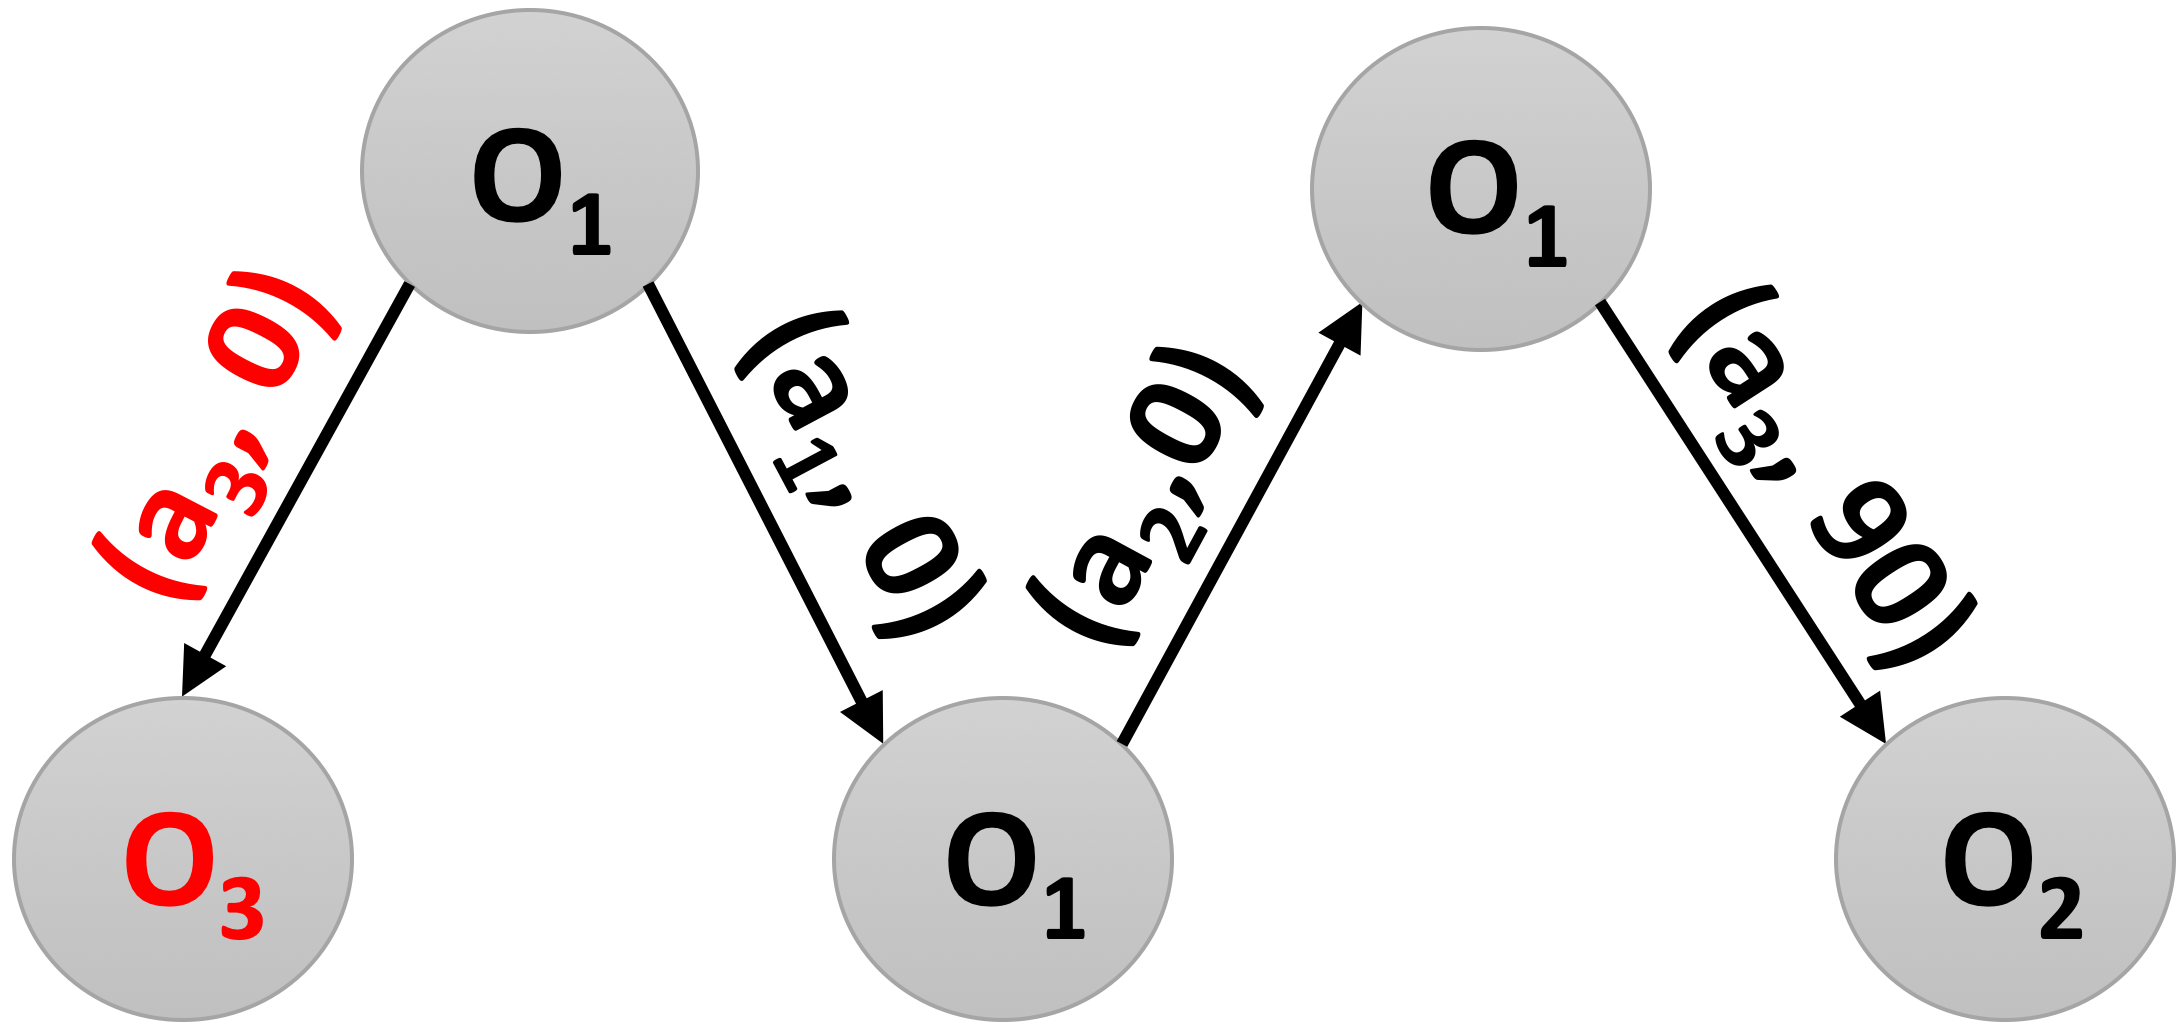
\includegraphics[width=0.45\textwidth]{Figures/problem.png}
%     \caption{The issue with using the number of different operations as observations. In order to achieve a reward of 90 the actions $a_1$ $\rightarrow$ $a_2$ $\rightarrow$ $a_3$ should be taken. But since the intermediate observations are similar and the intermediate rewards are 0, the network learns to apply $a_3$ directly and that $a_1$ and $a_2$ are ineffective. However, applying $a_3$ directly (as shown in red color) gives a reward of 0 and arrives at a different observation.}
%     \label{fig:problem1}
% \end{figure}


% To guarantee the observations change after applying each pass, and to enable operating on multiple programs simultaneously for efficiency, the actions were simply used as observations. In other words, the input of the network (observation) was defined as a histogram of the passes given so far and the passes were given an index from 0 to the number of passes. The output is the next pass to apply. This way the network can keep track of the passes given so far and learn which sequences should be applied to maximize the reward.


%(for example, in Figure~\ref{fig:problem1}, the actions $a_1$ and $a_2$ are effective but the network is blind to that because they contribute a zero reward). %The final algorithm is illustrated in figure~\ref{}.

\subsection{One-Hot Versus Histogram Representation}
% \begin{figure}
%     \centering
%     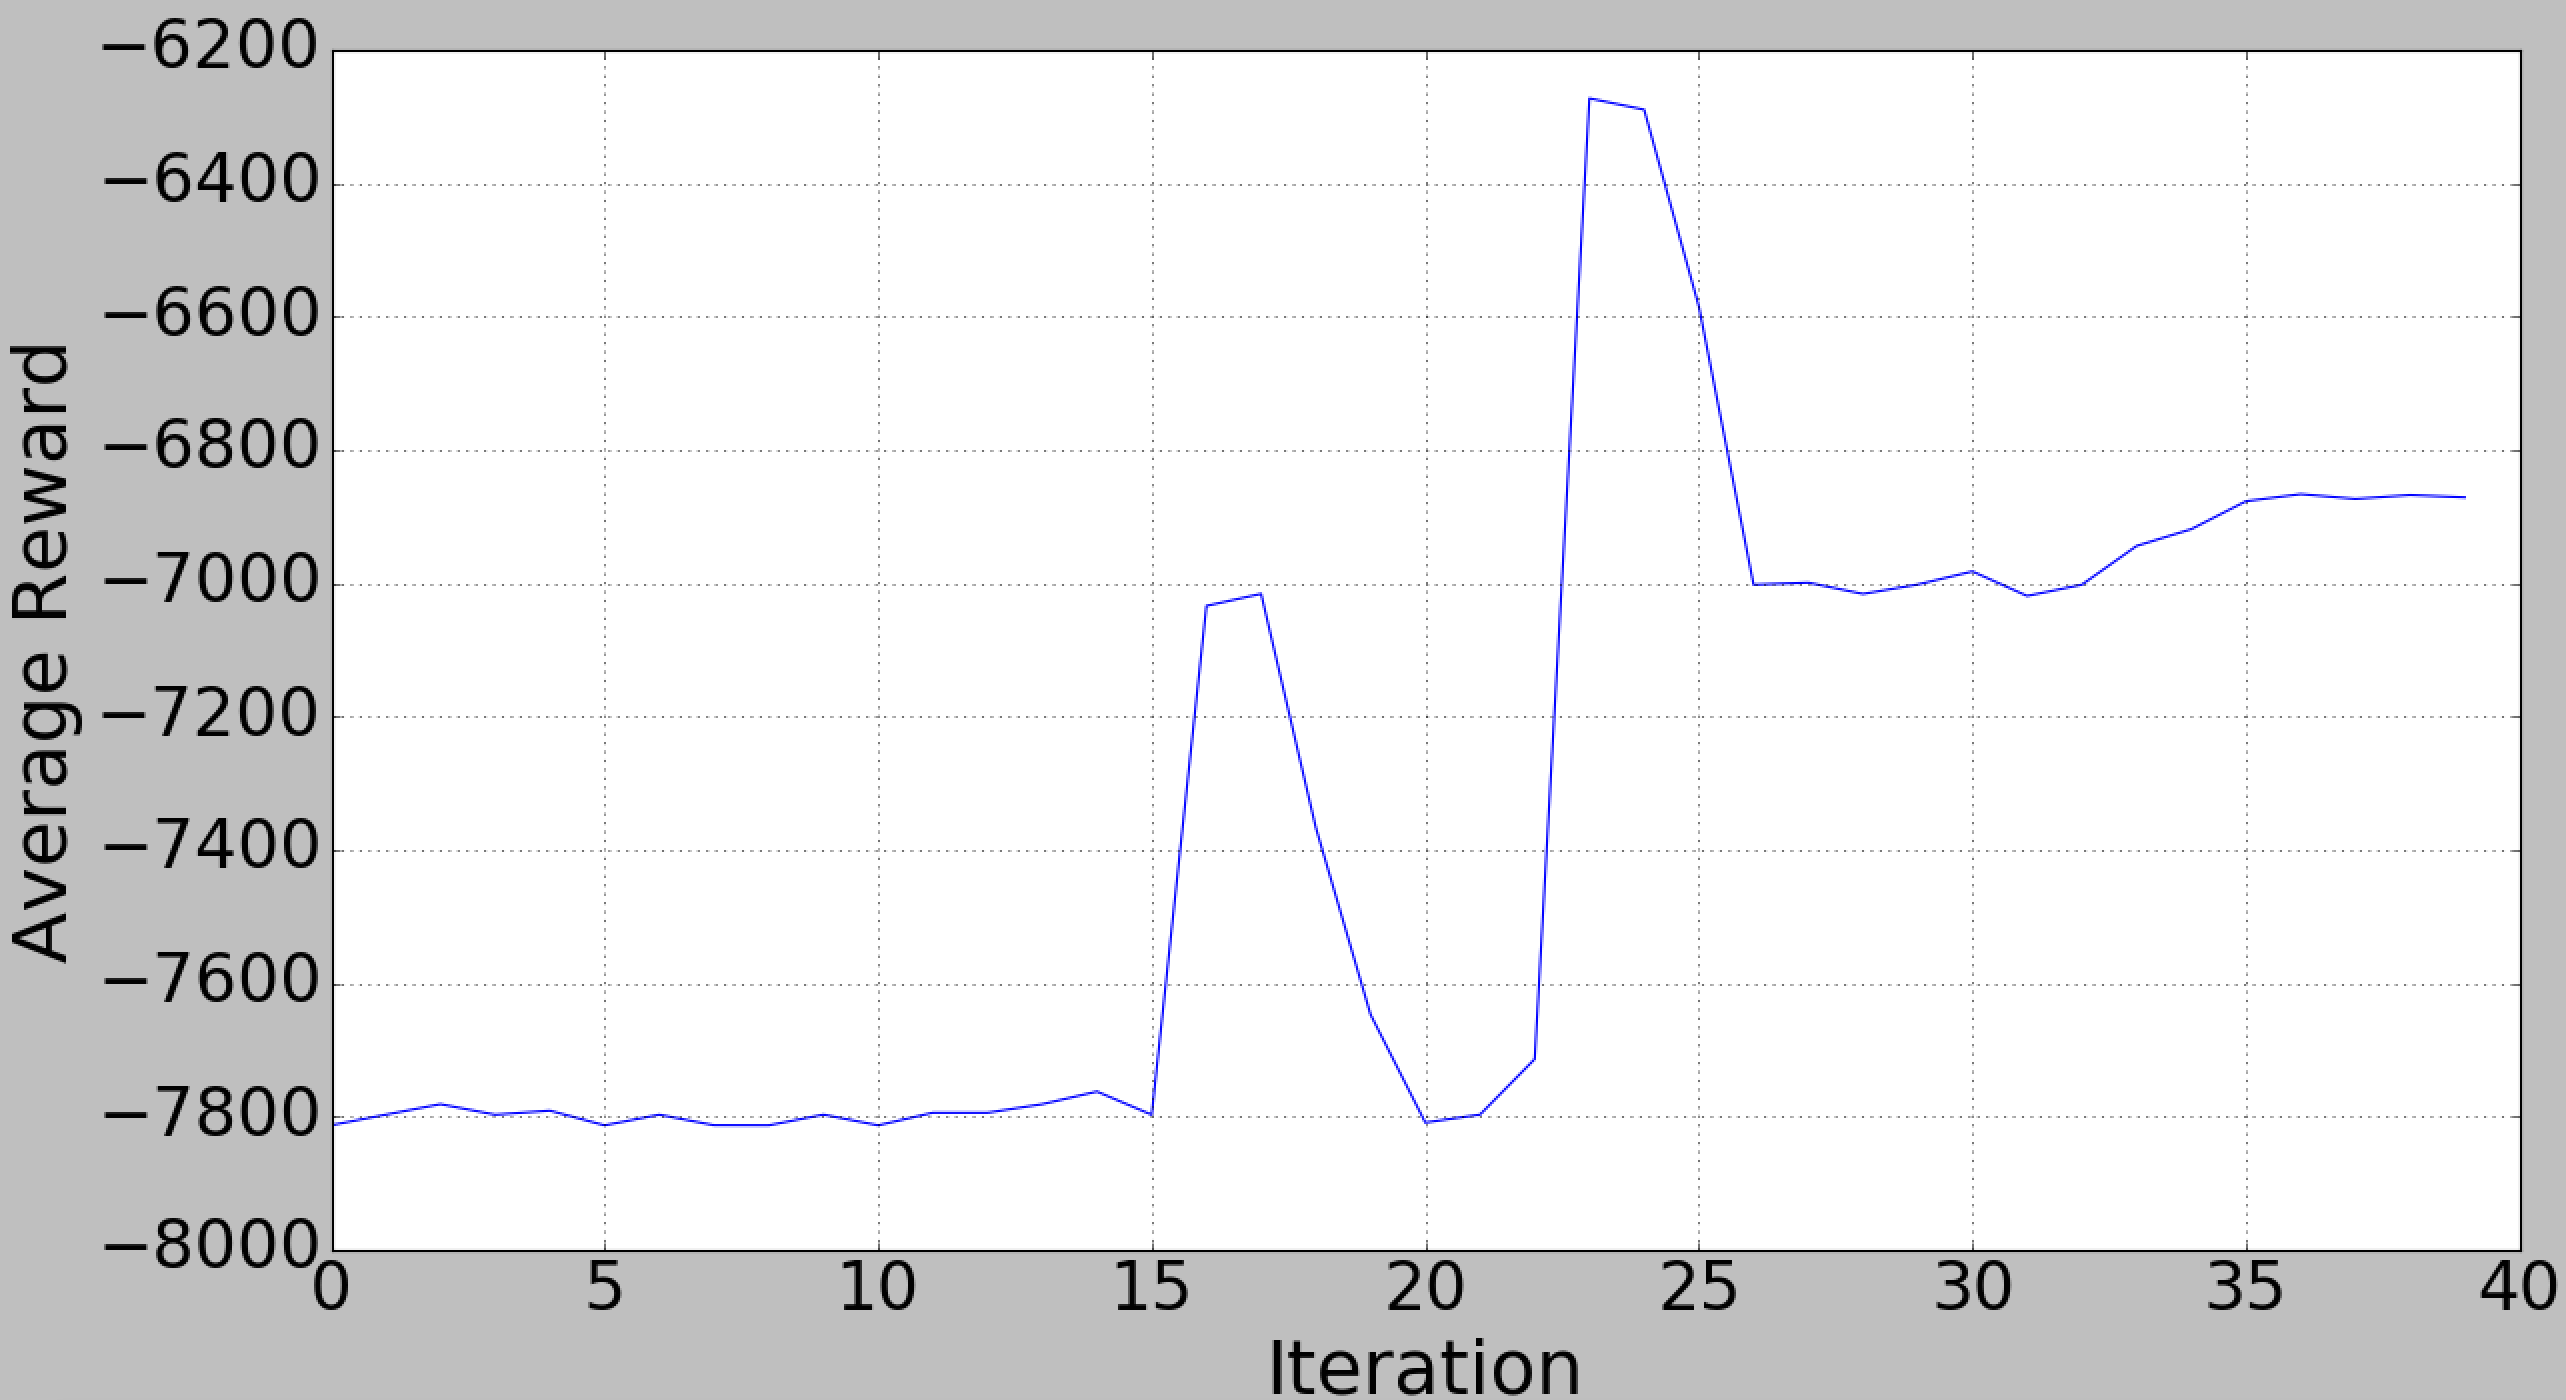
\includegraphics[width=0.5\textwidth]{Figures/gsmonlyhotone.png}    
%     \caption{The average reward (averaged over 50 steps) as a function of iteration for the gsm task. The maximum number of passes applied is five. The maximum reward achieved by the network is the global maximum possible with five passes.}
%     \label{fig:hotone}
% \end{figure}
% \begin{figure*}[!t]
%     \centering        
%     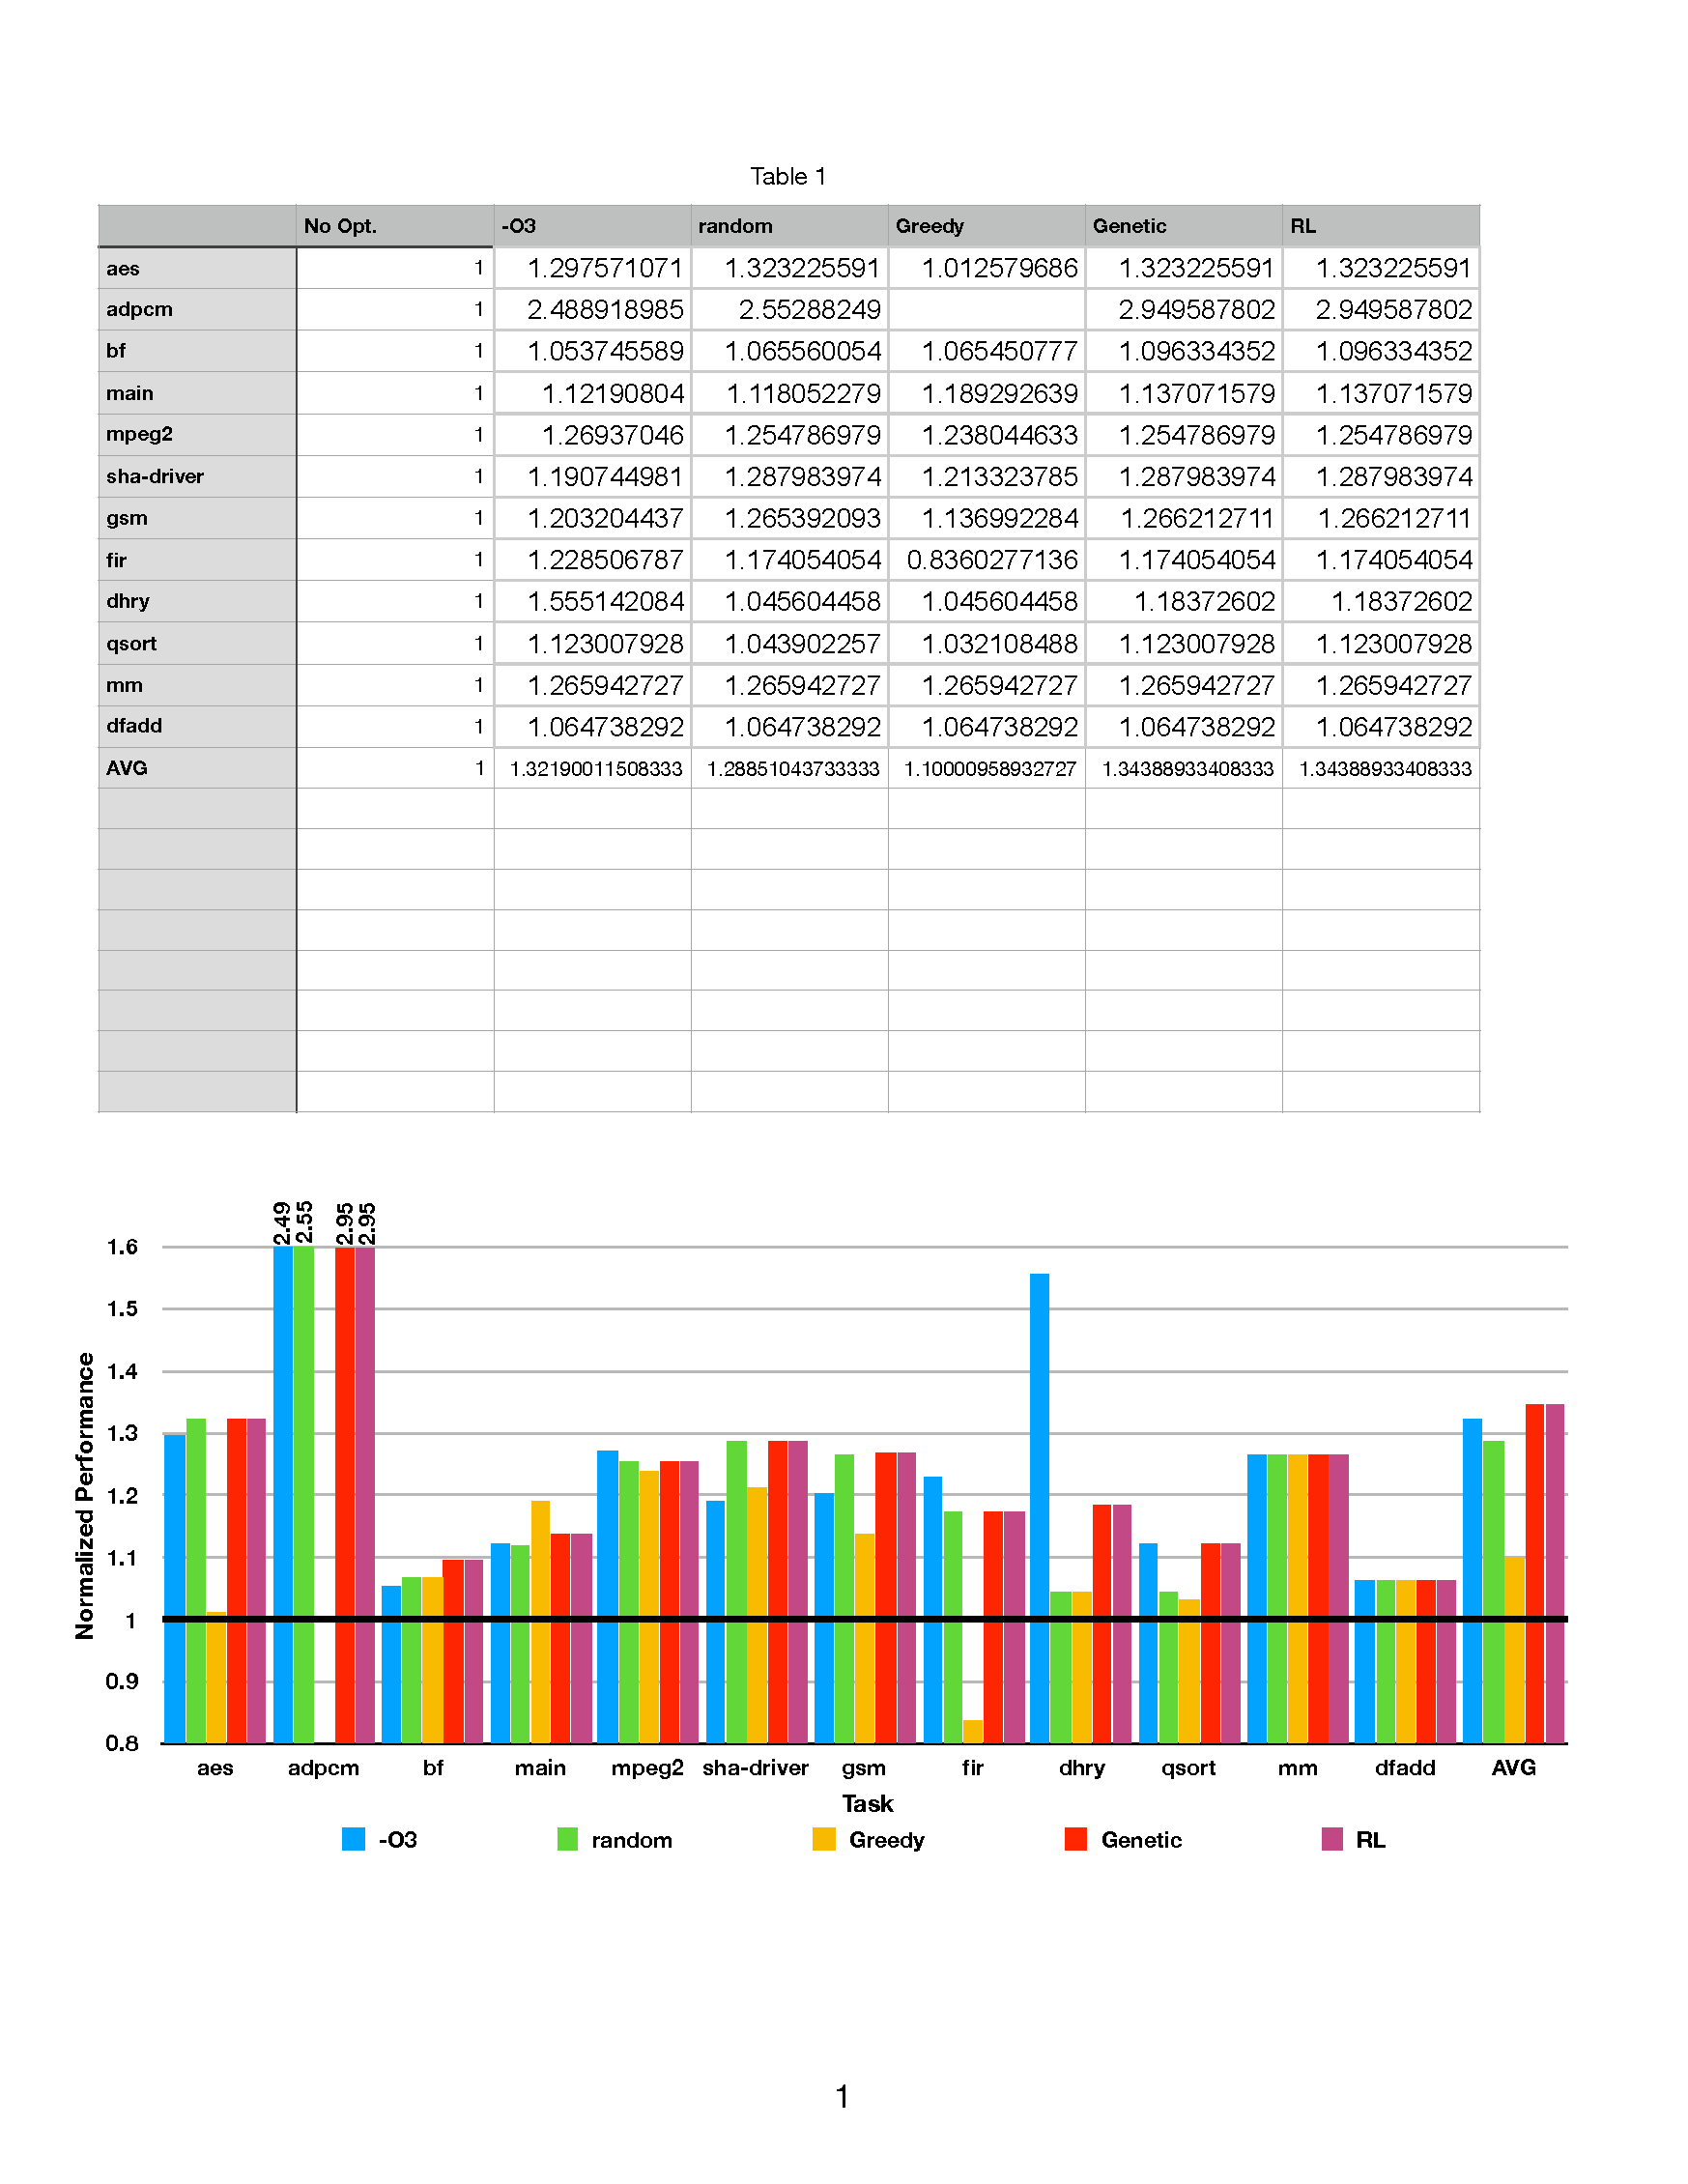
\includegraphics[trim={1.2cm 5.6cm 2cm 21cm},clip,width=\textwidth]{Figures/3passesv3.pdf} 
%     \caption{The performance for searching the best three passes using the different search algorithms for different tasks normalized to the case without any optimization. The exact number of cycles are listed in the appendix in Table~\ref{tab:3pass}}
%     \label{fig:3pass}
% \end{figure*}
Instead of using a histogram, a concatenation of $K$ one-hot vectors could be used, where $K$ is the number of passes to apply. The index $i$ of each vector$_j$ is $1$ if the $j^{th}$ pass applied is $i$, otherwise zero. This would allow RL to better understand the ordering of previously applied passes.
%The reward, for the hot one approach, on the gsm task, as a function of time step (averaged over 50 steps) is shown in Figure~\ref{fig:hotone}. The maximum number of passes applied is five. The network achieves the global maximum possible with five passes but it does not stabilize there. This could be due to the instability of DQN, network parameters, seeds, and large size of the network input observation. 
In practice, this did not improve performance largely because the state space is much larger, it takes a long time to learn. Moreover, increasing the maximum number of passes will make it effectively impossible for the network to learn. This is because adding one more pass requires adding $45$ inputs/features to the network (the total number of passes) making it more difficult for the network to converge.
\section{Results} % 2 pages 
\label{sec:results}
% \begin{table*}[!h]
% \caption{The runtime of the search algorithms for different number of passes.\TODO{billy: i think we'd save space by transposing this}}
% \label{tab:runtime}
% \hskip2.3cm\begin{tabular}{|c|c|c|c|c|c|c|c|c|}
% \hline
% \textbf{}          & \multicolumn{8}{c|}{\textbf{Runtime (minutes)}}                                                                                           \\ \hline
% \textbf{Task} & \textbf{Bruteforce} & \textbf{DQN} & \textbf{PG} & \textbf{-O3} & \textbf{random} & \textbf{Greedy} & \textbf{Genetic} & \textbf{No Opt.} \\ \hline
% \textbf{3 passes}  & 4725                & 44           & 49        & 0.1          & 4725            & 19              & 150             & 0.1              \\ \hline
% \textbf{12 passes} & 3.58E+18            & 31           & 21        & 0.1          & 360             & 222             & 411             & 0.1              \\ \hline
% \textbf{24 passes} & 2.46E+38            & 20           & 34        & 0.1          & 360             & 837             & 1017            & 0.1              \\ \hline
% \end{tabular}
% \end{table*}
% The algo shown in Fig 7 takes 1025mins to for 3 passes on 4 progs 
% 
\vspace{-0.1cm}
We implemented the framework in Python and TensorFlow~\cite{TF}. The network topology consisted of a $512\times256$ FC layer for the DQN, and $256\times256$ FC layer for the PG. We ran the framework on a four-core Intel i7-4765T CPU~\cite{Intel2017} with a Tesla K20c GPU~\cite{Nvidia2012} for handling the training and inference.
We use the number of clock cycles reported by the HLS profiler as the performance metric. 
In~\cite{huang2013effect}, results showed a one-to-one correspondence between the clock cycle count and the actual hardware execution time. Therefore, better clock cycle count will lead to better hardware performance. 
%We also validated the reported clock cycles with logic simulation. 

%Moreover, the clock cycle counts can be reported during the compile time within seconds, which allows us to generate adequate number of trajectories for RL\TODO{Ameer: Do we need this sentence? }. 
Success is defined as learning a sequence of passes that performs better than -O3 within a reasonable time. 
%This is mainly due to a compile time constraint imposed by the deep reinforcement learning algorithms. 
%The clock cycle counts can be reported by the HLS profiler during the compile time within seconds. 
%(which minimizes the number of cycles) based on the features extracted from the program. 
We use $12$ benchmarks for evaluation taken from CHstone~\cite{hara2008chstone} and LegUp examples. The benchmarks contain a variety of applications from different domains, such as arithmetic, media, and cryptography. The number of cycles required to run the benchmarks ranges from thousands to millions. We ran DQN and PG, and compared it against random search, greedy algorithms~\cite{huang2013effect}, genetic algorithms~\cite{DEAP_JMLR2012}, and -O3. All results are normalized to the case where no optimization was applied.
%It is written in a limited subset of standard C excluding the structures that are not commonly supported by the HLS tools, such as floating-point, struct composition, dynamic memory allocation and recursion. 
%All programs in the CHStone benchmark suite are synthesizable.

\subsection{Impact of the Sequence Length}
Figure \ref{fig:length} shows the circuit speedup for various algorithms with sequence lengths of 3, 12, and 24.  
For each algorithm, we set the optimization sequence to a fixed length.
The sequences for three passes are generated with each algorithm running to optimize for four programs. 
The sequences for 12 and 24 passes are generated with each algorithm optimizing six programs. 
We then applied the generated sequences to all 12 programs, normalized the results to the No-Opt performance, and  
took the average of the normalized performance for the 12 programs. 
Results show that three passes is not adequate to achieve peak performance for the 12 benchmarks. 

For DQN, PG, genetic and greedy algorithms, little performance improvement is observed by increasing the length from 12 to 24. 
With 24 passes, PG, DQN and Genetic algorithms perform better than the rest. 


%\subsection{3 Passes}
% \begin{figure*}[!t]
%     \centering        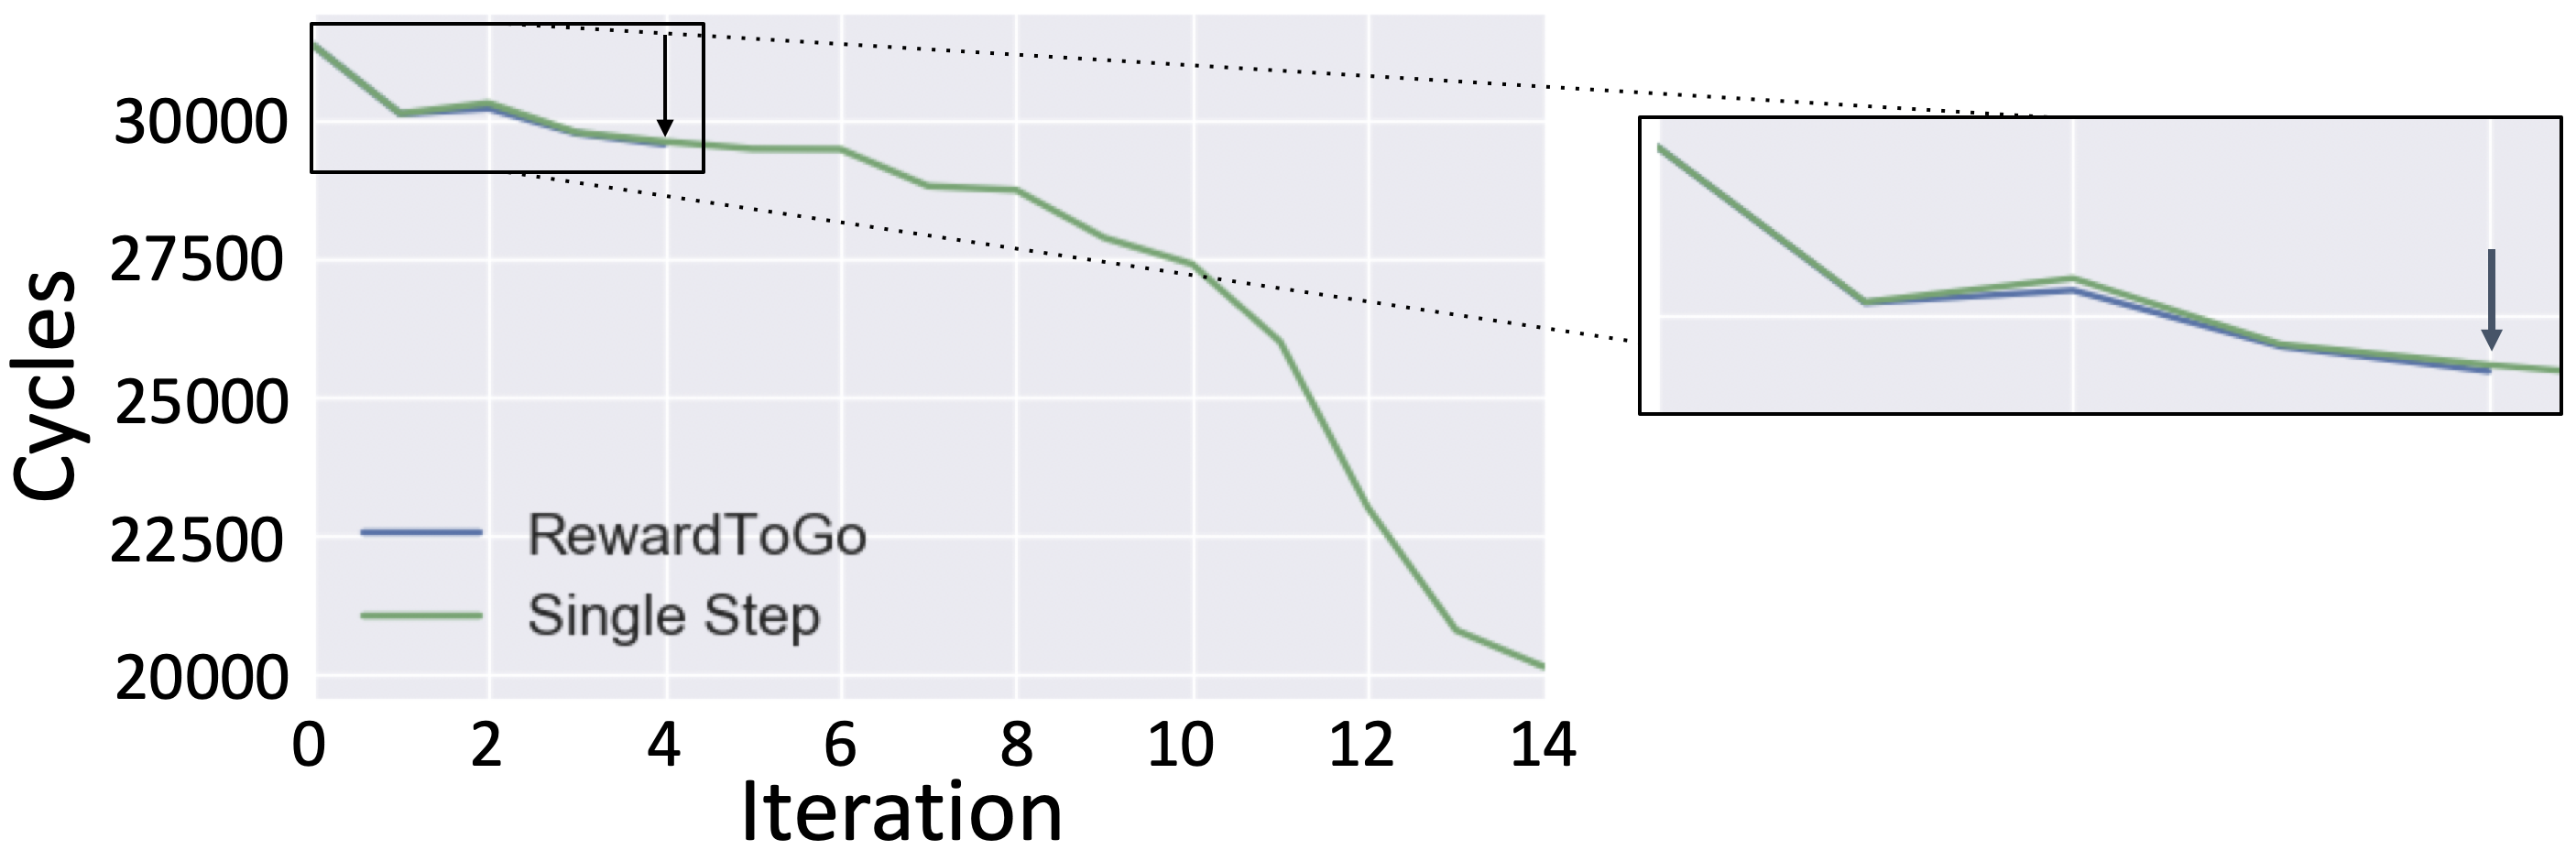
\includegraphics[width=\textwidth]{Figures/PG3passv2.png}    
%     \caption{The mean cycles as a function of timestep in the PG framework to find the three optimal passes.}
%     \label{fig:PG1}
% \end{figure*}

% \begin{figure}[!t]
%     \centering
%     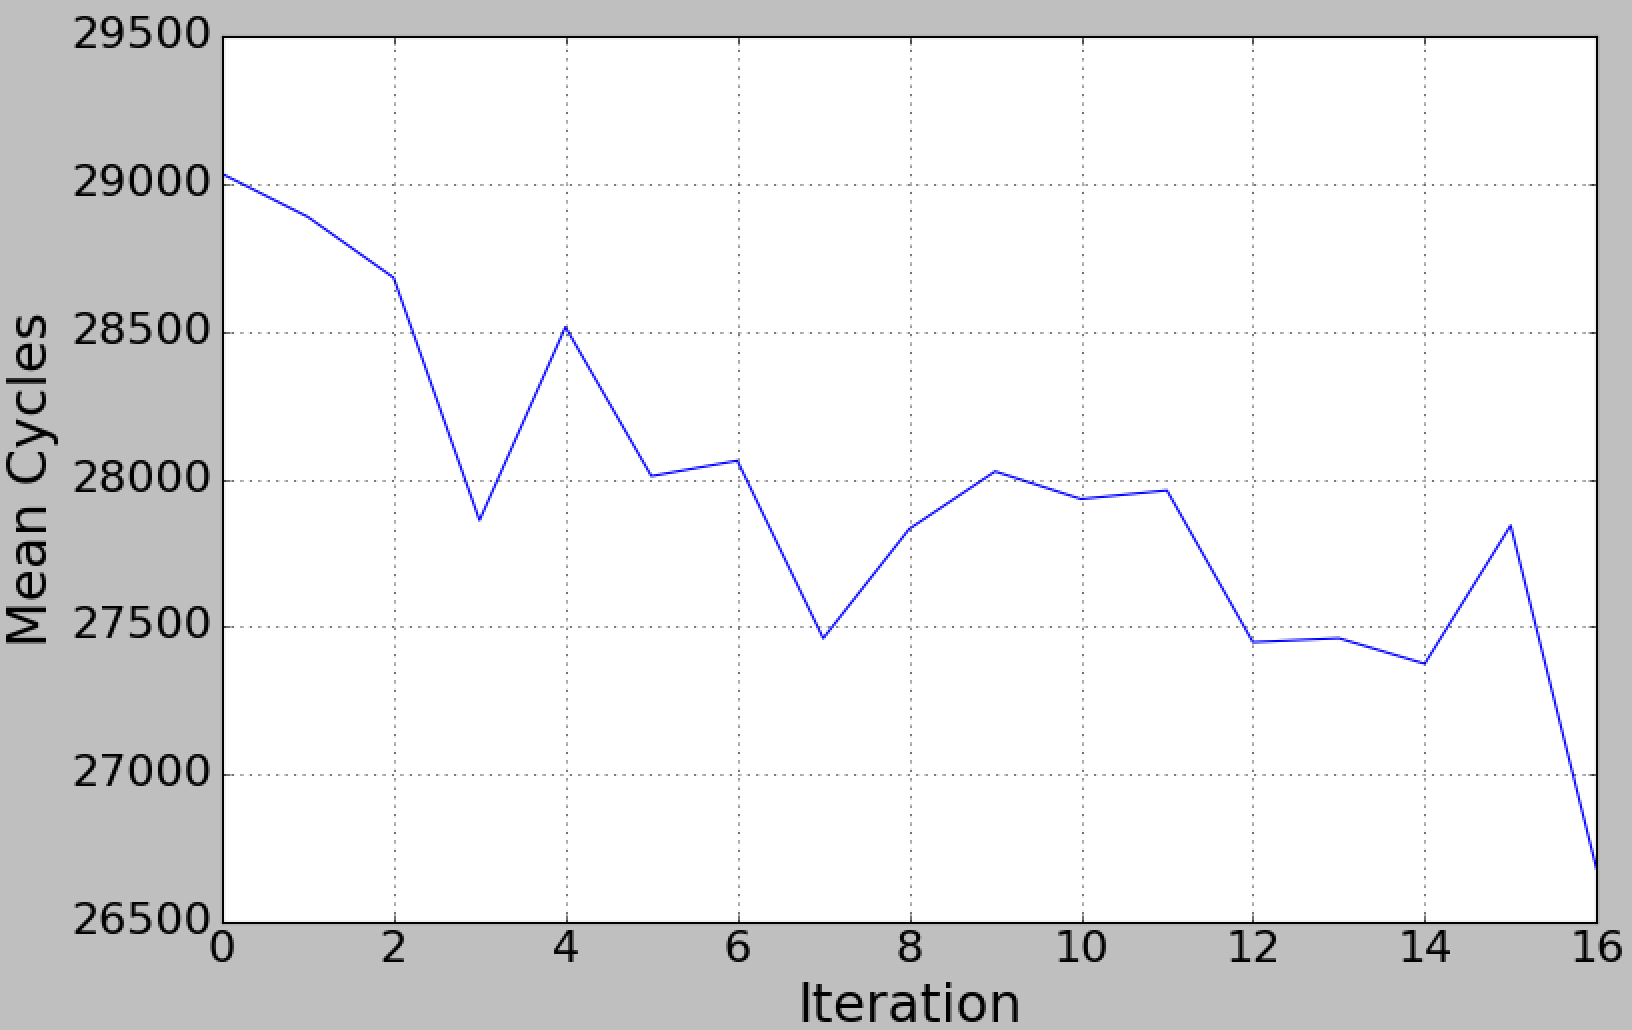
\includegraphics[width=0.5\textwidth]{Figures/dqn3pass.png}
%     \caption{The cycles as a function of timestep in the DQN framework to find the three optimal passes.}
%     \label{fig:dqn1}
% \end{figure}
%Our first evaluation is to evaluate the performance of the different search algorithms with a small number of passes
\begin{table}[!t]
\caption{The optimization time of the search algorithms for different number of passes.}
\vspace{-0.2cm}
\label{tab:runtime}
\begin{tabular}{|c|c|c|c|c|c|c|}
\hline
\textbf{}          & \multicolumn{6}{c|}{\textbf{Optimization Time (minutes)}}                                                                                           \\ \hline
\textbf{\hspace{-1.2mm}\# passes\hspace{-1.2mm}} & \textbf{\hspace{-1.2mm}Exhaustive\hspace{-1.2mm}} & \textbf{\hspace{-1.2mm}DQN\hspace{-1.2mm}} & \textbf{PG} & \textbf{\hspace{-1.2mm}Random\hspace{-1.2mm}} & \textbf{\hspace{-1.2mm}Greedy\hspace{-1.2mm}} & \textbf{\hspace{-1.2mm}Genetic\hspace{-1.2mm}} \\ \hline
\textbf{3 passes}  & 4725                & 44           & 49                & 4725            & 19              & 150                       \\ \hline
\textbf{12 passes} & 3.58E+18            & 31           & 21                & 360             & 222             & 411                      \\ \hline
\textbf{24 passes} & 2.46E+38            & 20           & 34             & 360             & 837             & 1017                    \\ \hline
\end{tabular}
\vspace{-0.5cm}
\end{table}

\subsection{Optimization Time Comparison}

Table~\ref{tab:runtime} lists the time it took to run each algorithm for differing number of passes. For three passes, it is possible to find the optimal sequence as the exhaustive-search is feasible. The exhaustive-search solution took $78.75$ hours to run. We ran the random search for $78.75$ hours, yet it did not find the optimal sequence. Also the greedy algorithm did not find this sequence.


The DQN, PG, and genetic algorithms quickly achieved this sequence. Additionally, DQN and PG achieved this sequence $3.4\times$ and $3.1\times$, respectively, faster than the genetic algorithm. To ensure  RL did not achieve the sequence by luck, we ran the RL framework ten times and verified that it derived the optimal ordering every time. Furthermore, we kept running the RL until it found the optimal sequence, although it found suboptimal ones much earlier. This is why it took more time to run the RL frameworks with three passes.
The optimal sequence was \textit{-simplifycfg, -loop-rotate}, and \textit{-loop-unroll}. Note that even with $3$ passes the performance of RL is 1.5\% better than -O3.
%For simplicity, we run the algorithms on four programs rather than twelve as these passes are optimal for most tasks. 
%Because of this, 
%The performance of the programs for the different search algorithms is shown in Figure~\ref{fig:3pass}. 
%By contrast, 

Results show that adding more passes resulted in a minor impact on optimization time for the RL algorithms but a major impact for the greedy and genetic algorithms. Note that for 12 and 24 passes, it would take more than one trillion years to run exhaustive-search. Therefore, the time given is an estimate based on the optimization time for three passes. Furthermore, we limited the time to run random search to six hours when applying 12 and 24 passes. Greedy and genetic algorithms run one to two orders of magnitude slower than the RL algorithms and achieve lower circuit performance for greedy algorithm and similar circuit performance for genetic algorithm. The algorithm optimization time benefits are mainly due to the data efficiency of the RL algorithms and the optimizations proposed in Section~\ref{sec:DRLA} that make it possible to significantly reduce the number of compilations required when running the framework and using the previously applied passes as the input observations. %The optimal sequence it arrived at was \textit{-sink, -loop-rotate}, and \textit{-loop-unroll}.  %which achieves 3.5\% lower performance than the optimal. Note that even with $3$ passes the performance of RL is 1.5\% better than -O3. The performance of RL is also 10\% better than greedy. The genetic algorithm was able to achieve similar results but in $3\times$ longer time. The runtimes are summarized in table~\ref{tab:runtime}. 

\begin{figure}[!t]
    \centering
    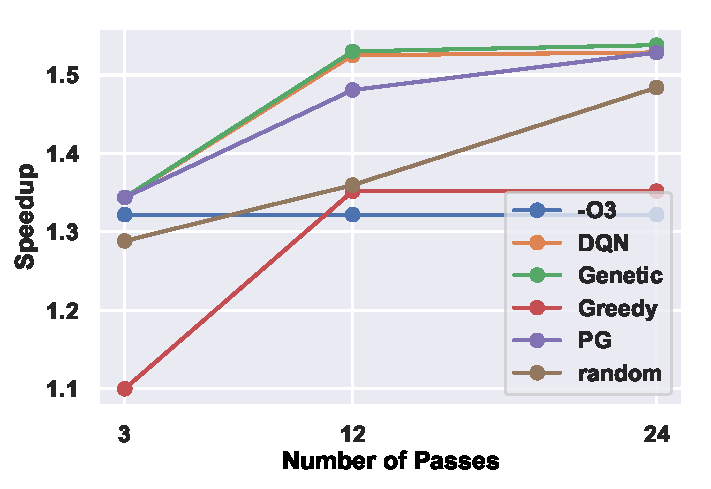
\includegraphics[width=0.5\textwidth]{Figures/length.pdf}
    \vspace{-0.7cm}
    \caption{Circuit speedup of various algorithms compared to No-Opt with sequence length of 3, 12, and 24.}
    \label{fig:length}
    \vspace{-0.5cm}
\end{figure}

% Figure~\ref{fig:PG1} shows the number of cycles as a  function of timestep for the PG algorithm. The graph shows two plots, one for the PG algorithm (Single Step) where we only compile once at the end of the roll-out and another (RewardToGo) for the PG algorithm where we compile once after each pass applied and use the reward to go~\cite{Baxter2001} to reduce variance and thus further improve its performance. Within the same time frame, it is evident that since we are optimizing three passes, the runtime improves by $3\times$ when using Single Step over RewardToGO and the performance it achieves is $40\%$ better performance. 
\begin{figure*}[!t]
    \centering        
    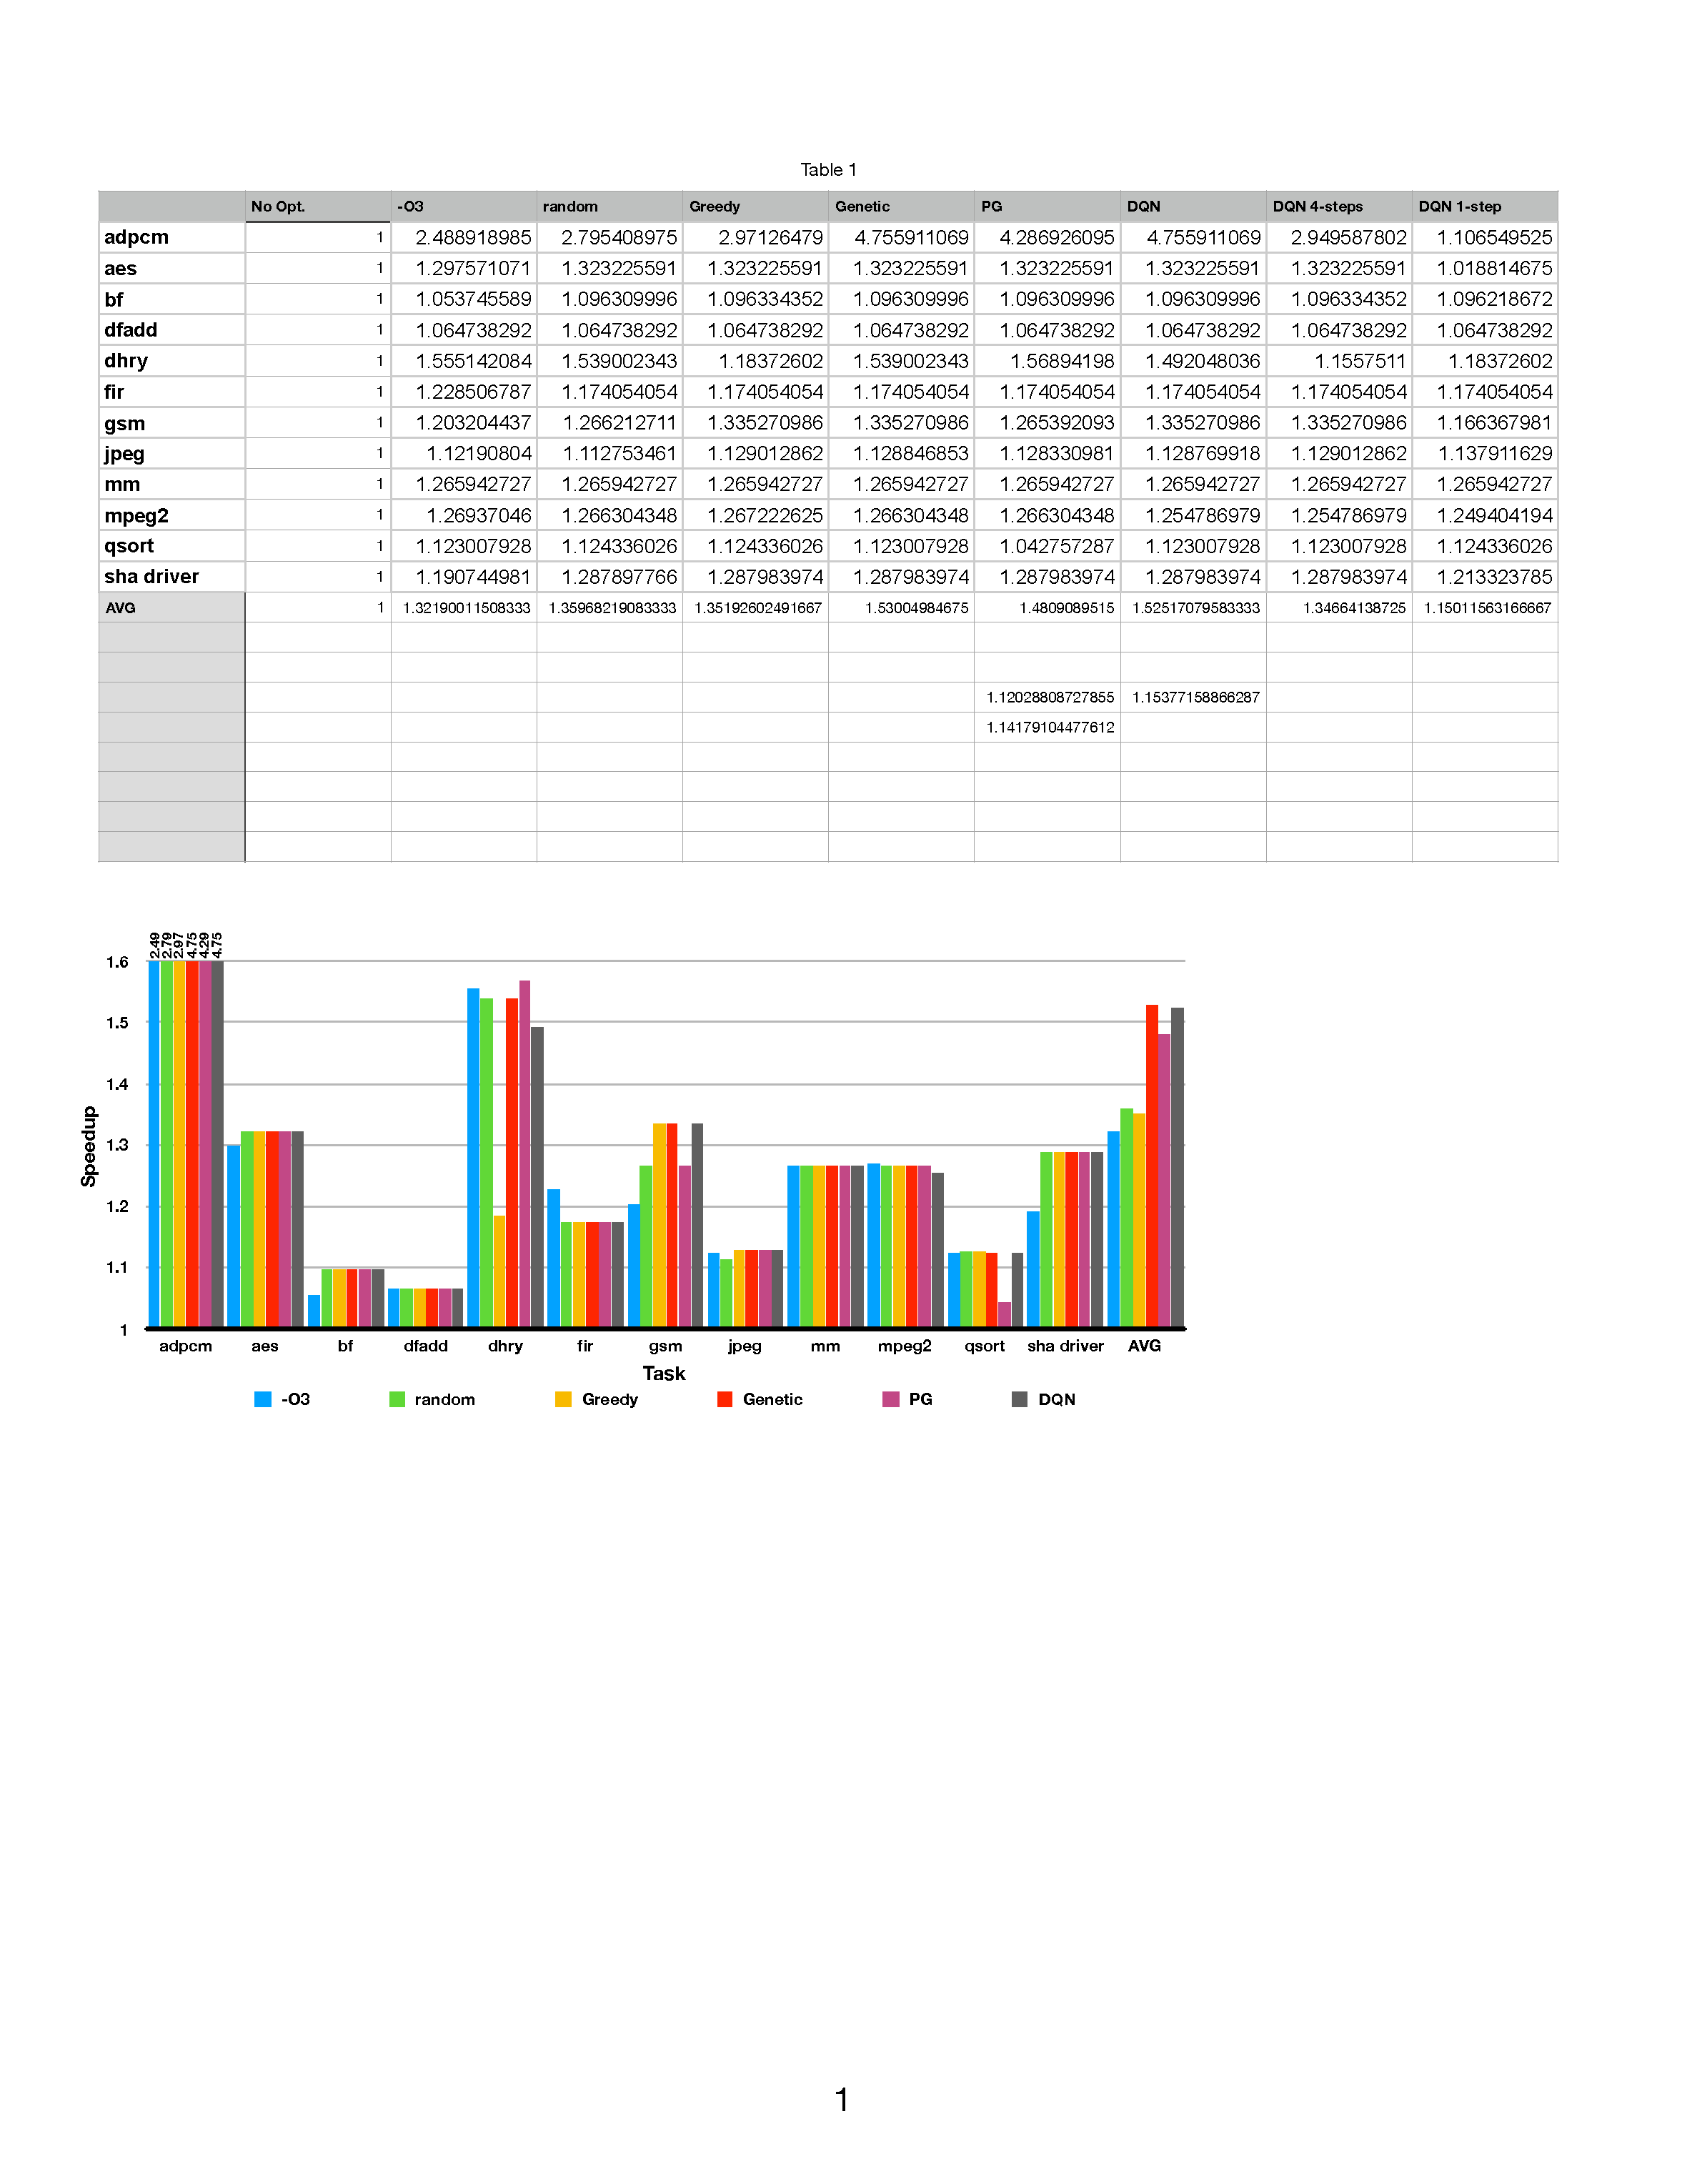
\includegraphics[trim={1.9cm 18cm 11.5cm 21.5cm},clip,width=\textwidth]{Figures/12passesv5.pdf} 
    \vspace{-0.7cm}
    \caption{The circuit speedup for searching the best 12 passes using the different search algorithms for different tasks normalized to the case without any optimization.%The exact number of cycles are listed in the appendix in Table~\ref{tab:12pass}
    }
    \label{fig:12pass}
    \vspace{-0.6cm}
\end{figure*}


% Figure \ref{fig:dqn1} shows the mean number of cycles as a function of timestep for the DQN algorithm. DQN runs much faster than PG. In all of our runs DQN found the optimal solution but it did not always stabilize there. But since we care only about a single good roll-out it was sufficient.

%\subsection{12 Passes}
\vspace{-0.1cm}
\subsection{Circuit Performance Comparison}
\vspace{-0.1cm}

Figure~\ref{fig:12pass} shows the circuit speedup of the different algorithms for finding the best $12$ passes as a function of time, normalized to No-Opt performance. The highest improvement is seen in DQN and genetic algorithms that both achieve $16\%$ better circuit speed over -O3 (six programs improved, three programs remained the same, and three programs worsened slightly). PG achieves $12\%$ better circuit speed over -O3. DQN requires less data to learn and this is why it achieves better speedup over PG. 
%Random search achieves slightly higher speedup than -O3, and greedy. This is mainly because we run it for a longer time and it runs more samples over time, as no training/processing is required on the data.


Figure~\ref{fig:12vstime} shows the geomean of circuit cycles of the programs as a function of time for genetic and greedy algorithms, and the average geomean of cycles for PG and DQN (averaged over batch size). For a fair comparison we cut the time after the algorithms stop improving. 
The greedy and genetic algorithms both have a large improvement at the beginning of the training phase because of its greedy nature. 
The greedy algorithm converges to a worse minimum result compared to the other algorithms, suggesting locally optimal choices may not be the best approach for tackling the phase-ordering problem. 
The genetic algorithm, however, has mutation, introducing randomness which helps to improve the performance. 
We see that both RL algorithms improve the average cycles of a batch over time. 

\subsection{Validation}
\vspace{-0.1cm}
After the framework finishes running on the LegUp simulator, we validate the cycle time results by compiling the generated Verilog and simulating the design with ModelSim. 
We see a 0.48\% difference between the actual and profiler-generated cycle time. 
We also compile all the optimized circuit designs with a standard FPGA toolflow and verify that frequency meets the 50 MHz constraint. We take the geomean across all the benchmarks for the area results. Compared to the -O3 area results, the DQN-optimized circuits have 0.6\%, 3\%, 43\% increase in LUTs, registers, and BRAMs respectively. The DSPs remained the same. Note that the objective of this paper is to optimize for circuit speed. Optimizing for area or both circuit speed and area is also feasible in a similar manner.
%\TODO{add area disimprovement}. 
%We now increase the number of passes to $12$. Note that a brute force solution would take more than one trillion years to run in that case. To see how well it scales we train on six programs and use these results to compile $12$ programs. The performance of the programs for the different search algorithms is shown in Figure~\ref{fig:12pass}. The runtimes are summarized in table~\ref{tab:runtime}. Three DQN results are presented: DQN $n$-steps where we compile once after applying $n$ passes and average the reward for $n=1,4,12$.  The highest performance is achieved in DQN $12$-steps and genetic algorithms that both achieved 16\% better performance than -O3, genetic, random and PG algorithms. Furthermore, DQN $12$-steps runs $7.1\times$ and $63\times$ faster than the greedy and genetic algorithms respectively. PG runs $10.5\times$ faster than greedy algorithms while achieving similar performance. 

\begin{figure}[!t]
    \centering
    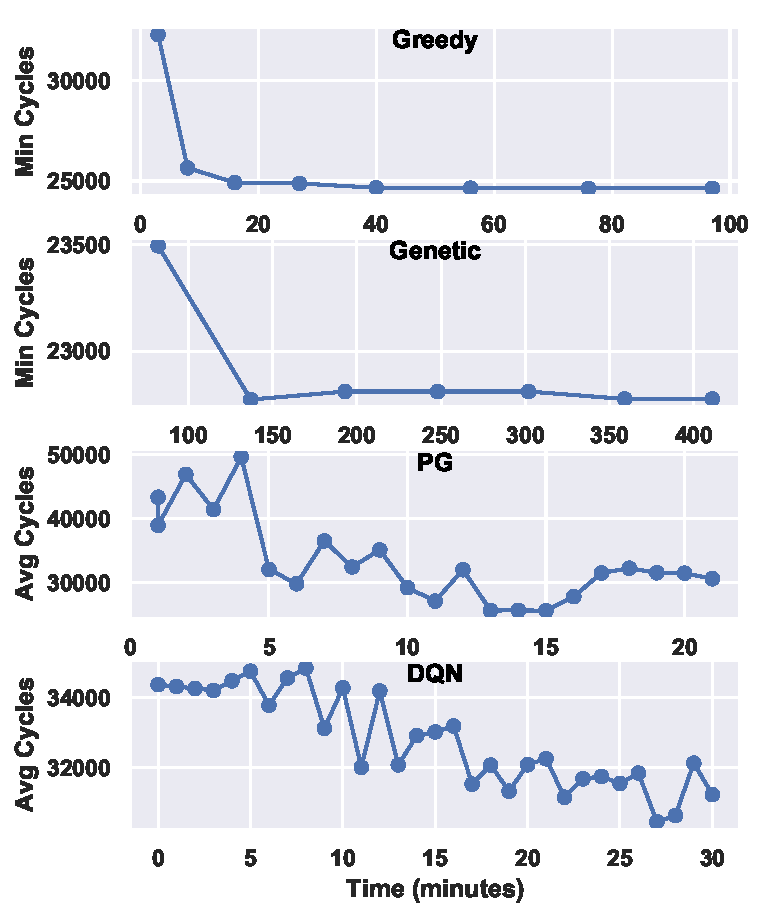
\includegraphics[trim={0cm 0cm 0cm 0.3cm},clip,width=0.5\textwidth]{Figures/12vstime.pdf}
    \vspace{-0.7cm}
    \caption{Geomean of circuit cycles for various algorithms as a function of algorithm training time.}
    \label{fig:12vstime}
    \vspace{-0.5cm}
\end{figure}

%\subsection{Impact on Generated Hardware}
%Table shows the actual cycle time of the programs. 
%\JENNY{Add tables}
%\subsection{Challenges and Discussion}
% \subsubsection{DQN $n$-steps}
% Figure~\ref{fig:dqn2} shows the mean cycles as a function of time step for the three DQN approaches. DQN $12$-steps is able to run more trajectories, explore more, take advantage of a larger batch size and find better results. On the other hand, it suffers from higher variance than DQN 4-steps and DQN 1-step, because the accuracy of the reward decreases when averaging over larger group of passes. DQN 4-steps  takes advantage of both exploration and lowered variance, but still achieves worse performance than DQN $12$-steps as it runs less trajectories in the same time frame. After running it for 15 additional minutes DQN $4$-steps achieved similar performance results to that of DQN $12$-steps. DQN $1$-step on the other hand has the least variance but since it runs very slow it explores less and requires much more time to run.

% \begin{figure}[!t]
%     \centering
%     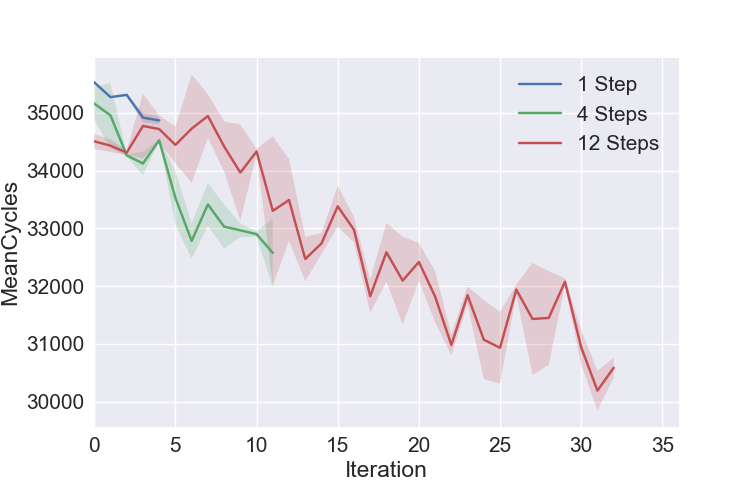
\includegraphics[width=0.5\textwidth]{Figures/dqn12pass.png}
%     \caption{The means cycles as a function of timestep in the DQN framework to find the $12$ optimal passes.}
%     \label{fig:dqn2}
% \end{figure}
% \subsubsection{PG vs. DQN}
% DQN is known to be more data efficient that PG \textit{i.e.,} require fewer samples than PG to learn. This is why DQN achieved better results than PG in similar time frames. Furthermore, DQN has more randomness/exploration part that allows it to explore more. Interestingly, the random search on $12$ passes achieved similar performance as PG, greedy and -O3 algorithms (although it took longer time to run). Given the large exploration space, the higher level of randomness in DQN gave it additional performance benefits.

% \subsubsection{Reward-to-go}     
% \begin{figure}[!t]
%     \centering
%     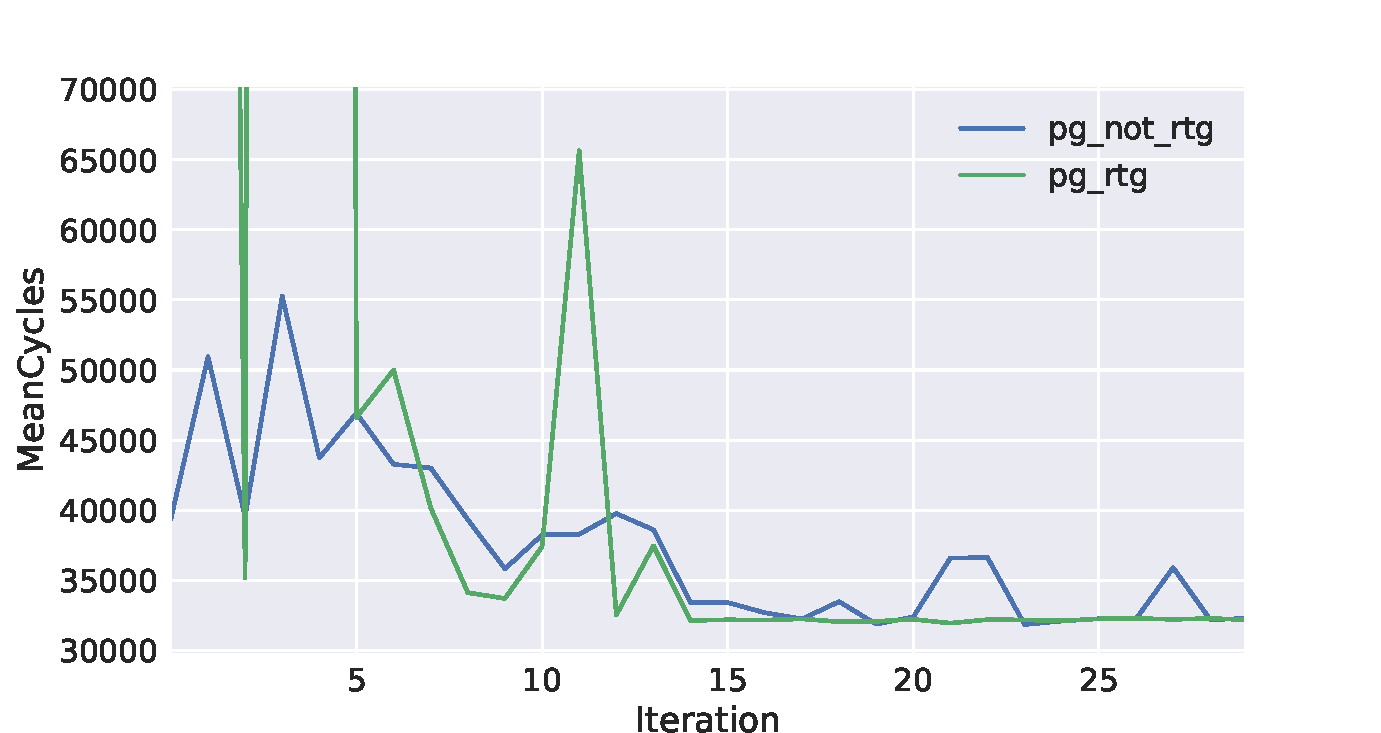
\includegraphics[width=0.5\textwidth]{Figures/pg_rtg_meancycle.pdf}
%     \caption{Mean Clock Cycles versus Training Iterations for Policy Gradient algorithms with and without Reward-to-go for a batch size of 100.}
%     \label{fig:pg_rtg}
% \end{figure}
% We run an experiment to compare the policy gradient with and without the use of reward-to-go for the $12$ passes with a batch size of 100. 
% %Instead of only running the simulator environment once after each trajectory with a fixed length is generated for reward estimation, we need to run the simulator environment every time after we apply a new pass to gather rewards for the neural network to learn the reward-to-go value function.
% While there is no significant difference in the final number of clock cycles shown in Figure~\ref{fig:pg_rtg} for both algorithms. Adding reward-to-go results in $11\times$ longer runtime (21 minutes vs 253  minutes). Thus, reward-to-go is not adopted in our algorithm to save the training time. 
% \subsubsection{PG Batch Size Sensitivity Analysis}
% Figure~\ref{fig:pg_batch} shows the learning curve of the policy gradient method with three different batch sizes: 100, 200 and 500. 
% We can see that the policy gradient converges to a lower minimum with larger batch sizes.
% However, the runtime of the algorithm for the same number of training iterations increases with the batch size. The training time is 21 minutes, 41 minutes and 103 minutes respectively. 

%\subsubsection{Trajectory}
%The maximum trajectory length used in this work is $12$ passes. This is due to the limited resources and time to generate the results that consume time which increases exponentially with the number of passes applied. Nevertheless, we ran some experiments of up to $96$ passes and realized the performance improvements in all the algorithms is up to 3\% in the best case while the runtime could extend to multiple days. We also tried using -O3 as a pass that the RL can choose to apply, but the results did not change.

\subsection{Possible Alternative Machine Learning Algorithms}
\vspace{-0.1cm}
Inspired by the observed advantage of randomness in random search, genetic algorithm, and DQN that enables more exploration, as well as the redundancy of observations, we believe other techniques such as Bandits~\cite{chapelle2011}, Exploration~\cite{bellemare2016}, Proximal Policy Gradients~\cite{schulman2017proximal}, and Evolution Strategies~\cite{salimans2017evolution} might also be good candidates to explore. These works leverage a great deal of randomness and exploration while maximizing rewards. Furthermore, it might be beneficial to combine the applied optimizations and program features as observations to the RL so it could benefit from both representations of the state.
% \begin{figure}[!t]
%     \centering
%     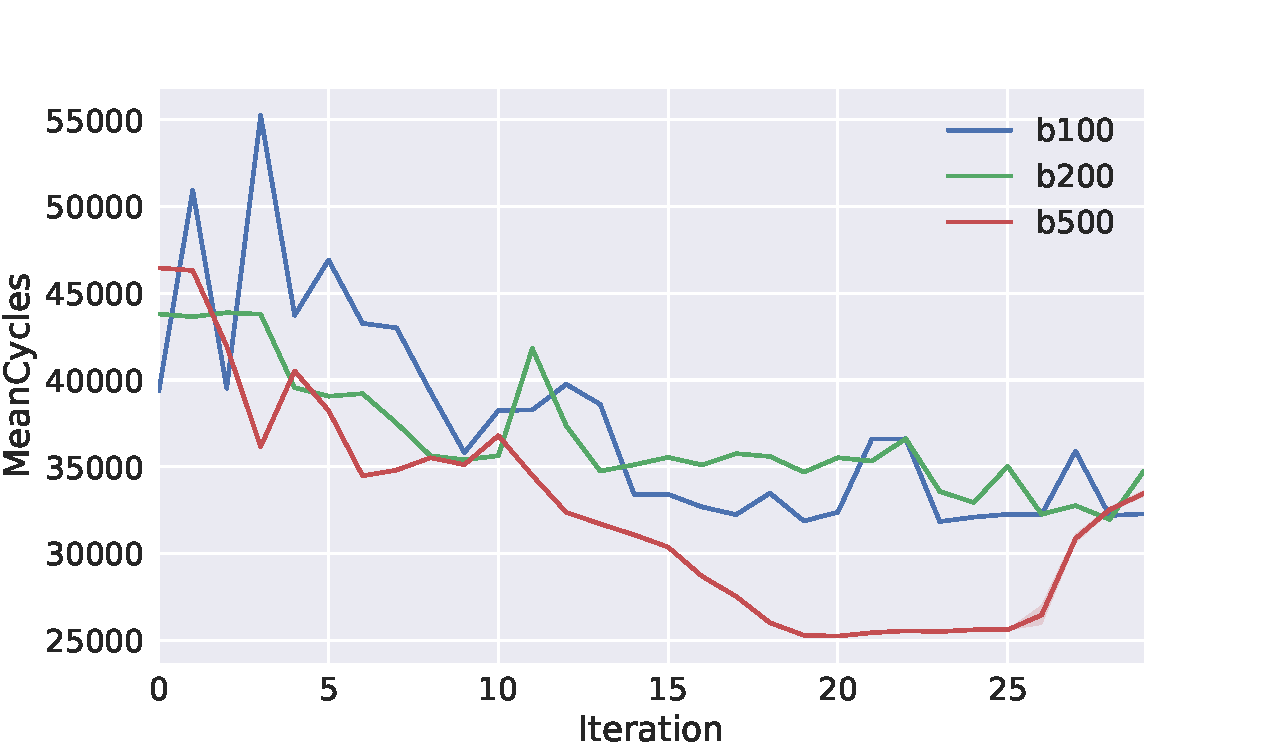
\includegraphics[width=0.5\textwidth]{Figures/pg_batch_meancycle.pdf}
%     \caption{Mean Clock Cycles versus Training Iterations for Policy Gradient algorithms with different batch sizes.}
%     \label{fig:pg_batch}
% \end{figure}
%\item Comparison among different ML algorithms 
%    \subitem put the table from midterm report 
\section{Conclusions} % 0.25 page 
\label{sec:conc}
\vspace{-0.1cm}
% In this work, we demonstrated a novel deep reinforcement learning based approach to robustly and intelligently improve the performance of HLS designs, by optimizing the compiler phase ordering. 
% These performance improvements require only a few minutes of training---one to two orders of magnitude faster than state-of-the-art approaches. 
% \JENNY{Add some numbers, how much better?}
% The techniques can be applied to software programs. 
% %The flexibility of our framework enables it to support optimizing any compiled program without being restricted to HLS. 
% We envision using such a framework to optimize a wide range of programs. 

In this work, we demonstrate a novel deep reinforcement learning based approach to improve performance of HLS designs by optimizing the compiler phase ordering. 
RL techniques achieve 16\% better results than traditional -O3 results. 
Such improvements require only a few minutes of training---one to two orders of magnitude faster than state-of-the-art approaches based on genetic algorithms.
While in this paper, we applied the techniques to HLS, the same RL techniques and framework can also be applied to software compilation and optimization.  

%In this work, we show the potential of using RL to achieve a better ordering of compiler optimization passes. We built a framework that takes multiple programs and intelligently and robustly finds an optimal sequence of passes to apply. 
%We also show that using the program features solely is insufficient for RL to learn, due to limited observations, the necessity to apply multiple passes sometimes to affect such features, and inability to operate on multiple programs simultaneously.
%We propose to use program features or the applied passes as observations. 
%Significant performance and runtime benefits are achieved by using the later approach.
%allowing a novel approach based on RL to tackle the compiler phase ordering challenge and opening new horizons to explore in RL where actions could be used as observations. %More work should be done to better represent the programs.

\bibliographystyle{IEEEtran}
\bibliography{projBib}

\appendices
\begin{table*}[!t]
\centering
\caption{Program features: number of different operations.}
\begin{tabular}{|c|c|}
\hline
Number of BB where total args for phi nodes \textgreater 5 & Number of And insts \\ \hline
Number of BB where total args for phi nodes is {[}1,5{]} & Number of BB's with instructions between {[}15,500{]} \\ \hline
Number of BB's with 1 predecessor & Number of BB's with less than 15 instructions \\ \hline
Number of BB's with 1 predecessor and 1 successor & Number of BitCast insts \\ \hline
Number of BB's with 1 predecessor and 2 successors & Number of Br insts \\ \hline
Number of BB's with 1 successor & Number of Call insts \\ \hline
Number of BB's with 2 predecessors & Number of GetElementPtr insts \\ \hline
Number of BB's with 2 predecessors and 1 successor & Number of ICmp insts \\ \hline
Number of BB's with 2 predecessors and successors & Number of LShr insts \\ \hline
Number of BB's with 2 successors & Number of Load insts \\ \hline
Number of BB's with \textgreater{}2 predecessors & Number of Mul insts \\ \hline
Number of BB's with Phi node \# in range (0,3{]} & Number of Or insts \\ \hline
Number of BB's with more than 3 Phi nodes & Number of PHI insts \\ \hline
Number of BB's with no Phi nodes & Number of Ret insts \\ \hline
Number of Phi-nodes at beginning of BB & Number of SExt insts \\ \hline
Number of branches & Number of Select insts \\ \hline
Number of calls that return an int & Number of Shl insts \\ \hline
Number of critical edges & Number of Store insts \\ \hline
Number of edges & Number of Sub insts \\ \hline
Number of occurrences of 32-bit integer constants & Number of Trunc insts \\ \hline
Number of occurrences of 64-bit integer constants & Number of Xor insts \\ \hline
Number of occurrences of constant 0 & Number of ZExt insts \\ \hline
Number of occurrences of constant 1 & Number of basic blocks \\ \hline
Number of unconditional branches & Number of instructions (of all types) \\ \hline
Number of Binary operations with a constant operand & Number of memory instructions \\ \hline
Number of AShr insts & Number of non-external functions \\ \hline
Number of Add insts & Total arguments to Phi nodes \\ \hline
Number of Alloca insts & Number of Unary operations \\ \hline
\end{tabular}
\label{tab:tab1}
\end{table*}

\begin{table*}[!t]
\caption{The cycles for searching the best three passes using the different search algorithms for different tasks.}
\label{tab:3pass}
\hskip3.3cm\begin{tabular}{|c|c|c|c|c|c|c|}
\hline
\textbf{\textbf{}}  & \multicolumn{6}{c|}{\textbf{Cycles}}                                                                                                                                                                \\ \hline
\textbf{Task}       & \textbf{RL}        & \textbf{-O3}      & \textbf{random}    & \textbf{Greedy}     & \textbf{Genetic} & \textbf{No Opt.} \\ \hline
\textbf{aes}        & \textcolor{blue}{9003}   & 9181                               & \textcolor{blue}{9003}   & 11765                                & \textcolor{blue}{9003}                              & 11913   \\ \hline
\textbf{adpcm}      & \textcolor{blue}{13707}  & 16244                              & 15837                               & Error                                   & \textcolor{blue}{13707}                               & 40430   \\ \hline
\textbf{bf}         & \textcolor{blue}{180050} & 187327                             & 185250                              & 185269                               & \textcolor{blue}{180050}                              & 197395  \\ \hline
\textbf{jpeg}       & 1296330                             & 1313851                            & 1318382                             & \textcolor{blue}{1239409} & 1296330                              & 1474020 \\ \hline
\textbf{mpeg2}      & 8356                                & \textcolor{blue}{8260}  & 8356                                & 8469                                 & 8356                              & 10485   \\ \hline
\textbf{sha driver} & \textcolor{blue}{209154} & 226234                             & \textcolor{blue}{209154} & 222024                               & \textcolor{blue}{209154}                               & 296387  \\ \hline
\textbf{gsm}        & \textcolor{blue}{6168}   & 6491                               & 6172                                & 6869                                 & \textcolor{blue}{6168}                               & 7810    \\ \hline
\textbf{fir}        & 1850                                & \textcolor{blue}{1768}  & 1850                                & 2598                                 & 1850                              & 2172    \\ \hline
\textbf{dhry}       & 7767                                & \textcolor{blue}{5912}  & 8793                                & 8793                                 & 7767                              & 9194    \\ \hline
\textbf{qsort}      & \textcolor{blue}{49948}  & \textcolor{blue}{49948} & 53733                               & 54347                                & \textcolor{blue}{49948}                              & 56092   \\ \hline
\textbf{mm}         & \textcolor{blue}{33244}  & \textcolor{blue}{33244} & \textcolor{blue}{33244}  & \textcolor{blue}{33244}   & \textcolor{blue}{33244}                              & 42085   \\ \hline
\textbf{dfadd}      & \textcolor{blue}{726}    & \textcolor{blue}{726}   & \textcolor{blue}{726}    & \textcolor{blue}{726}     & \textcolor{blue}{726}                              & 773     \\ \hline
\end{tabular}
\end{table*}

\begin{table*}[]
\caption{The cycles for searching the best $12$ passes using the different search algorithms for different tasks.}
\label{tab:12pass}
\hskip0.3cm\begin{tabular}{|c|c|c|c|c|c|c|c|c|c|}
\hline
\textbf{}                            & \multicolumn{9}{c|}{\textbf{Cycles}}                             
\\ \hline
\textbf{Task}       & \textbf{DQN 12-steps} & \textbf{DQN 4-steps} & \textbf{DQN 1-step} & \textbf{PG}   & \textbf{-O3}      & \textbf{random}   & \textbf{Greedy}    & \textbf{Genetic}   & \textbf{No Opt.} \\ \hline
\textbf{aes}        & \textcolor{blue}{9003}      & \textcolor{blue}{9003}     & 11693                                 & \textcolor{blue}{9003}  & 9181                               & \textcolor{blue}{9003}  & \textcolor{blue}{9003}   & \textcolor{blue}{9003}      & 11913                             \\ \hline
\textbf{adpcm}      & \textcolor{blue}{8501}      & 13707                                 & 36537                                 & 13657                           & 16244                              & 14463                              & 13607                               & \textcolor{blue}{8501}   & 40430                             \\ \hline
\textbf{bf}         & 180054                                 & \textcolor{blue}{180050}   & 180069                                & \textcolor{blue}{180050}                           & 187327                             & 180054                             & \textcolor{blue}{180050} & 180054                              & 197395                            \\ \hline
\textbf{jpeg}       & 1305864                                & 1305583  & \textcolor{blue}{1295373}  & 1296330                           & 1313851                            & 1324660                            & 1305583                             & 1305775                             & 1474020                           \\ \hline
\textbf{mpeg2}      & 8356                                   & 8356                                  & 8392                                  & 8280                           & \textcolor{blue}{8260}  & 8280                               & 8274                                & 8280                                & 10485                             \\ \hline
\textbf{sha driver} & \textcolor{blue}{209154}    & \textcolor{blue}{209154}   & 222024                                & \textcolor{blue}{209154}                          & 226234                             & 209168                             & \textcolor{blue}{209154} & \textcolor{blue}{209154} & 269387                            \\ \hline
\textbf{gsm}        & \textcolor{blue}{5849}      & \textcolor{blue}{5849}     & 6696                                  & 6168                           & 6491                               & 6168                               & \textcolor{blue}{5849}   & \textcolor{blue}{5849}   & 7810                              \\ \hline
\textbf{fir}        & 1850                                   & 1850                                  & 1850                                  & 1850                           & \textcolor{blue}{1768}  & 1850                               & 1850                                & 1850                                & 2172                              \\ \hline
\textbf{dhry}       & 6162                                   & 7955                                  & 7767                                  & 7767                           & \textcolor{blue}{5912}  & 5974                               & 7767                                & 5974                                & 9194                              \\ \hline
\textbf{qsort}      & \textcolor{blue}{49948}     & \textcolor{blue}{49948}    & 49889                                 & \textcolor{blue}{49948}                           & \textcolor{blue}{49948} & 49889                              & 49889                               & \textcolor{blue}{49948}  & 56092                             \\ \hline
\textbf{mm}         & \textcolor{blue}{33244}     & \textcolor{blue}{33244}    & 33244                                 & \textcolor{blue}{33244}                           & \textcolor{blue}{33244} & \textcolor{blue}{33244} & \textcolor{blue}{33244}  & \textcolor{blue}{33244}  & 42085                             \\ \hline
\textbf{dfadd}      & \textcolor{blue}{726}       & \textcolor{blue}{726}      & 726                                   & \textcolor{blue}{726}                           & \textcolor{blue}{726}   & \textcolor{blue}{726}   & \textcolor{blue}{726}    & \textcolor{blue}{726}    & 773                               \\ \hline
\end{tabular}
\end{table*}

% \begin{table}[]
% \begin{tabular}{|c|c|c|c|c|c|c|}
% \hline
% \textbf{\textbf{}}  & \multicolumn{6}{c|}{\textbf{Cycles}}                                                                                                                                                                                                                                   \\ \hline
% \textbf{Task}       & \textbf{RL}                 & \textbf{-O3}              & \textbf{random}           & \textbf{Greedy}            & \textbf{Genetic}           & \textbf{No Opt.} \\ \hline
% \textbf{aes}        & \textcolor{blue}{9003}    & 9181                                       & \textcolor{blue}{9003}  & \textcolor{blue}{9003}   & \textbf{9003}              & 11913                             \\ \hline
% \textbf{adpcm}      & \textcolor{blue}{8501}    & 16244                                      & 14463                                      & 13607                                       & \textcolor{blue}{8501}   & 40430                             \\ \hline
% \textbf{bf}         & \textcolor{blue}{180050}  & 187327                                     & 180054                                     & \textcolor{blue}{180050} & 180054                                      & 197395                            \\ \hline
% \textbf{jpeg}       & \textcolor{blue}{1295373} & 1313851                                    & 1324660                                    & 1305583                                     & 1305775                                     & 1474020                           \\ \hline
% \textbf{mpeg2}      & 8356                                         & \textcolor{blue}{8260}  & 8280                                       & 8274                                        & 8280                                        & 10485                             \\ \hline
% \textbf{sha driver} & \textcolor{blue}{209154}  & 226234                                     & 209168                                     & \textcolor{blue}{209154} & \textcolor{blue}{209154} & 269387                            \\ \hline
% \textbf{gsm}        & \textcolor{blue}{5849}    & 6491                                       & 6168                                       & \textcolor{blue}{5849}   & \textcolor{blue}{5849}   & 7810                              \\ \hline
% \textbf{fir}        & 1850                                         & \textcolor{blue}{1768}  & 1850                                       & 1850                                        & 1850                                        & 2172                              \\ \hline
% \textbf{dhry}       & 6162                                         & \textcolor{blue}{5912}  & 5974                                       & 7767                                        & 5974                                        & 9194                              \\ \hline
% \textbf{qsort}      & \textcolor{blue}{49948}   & \textcolor{blue}{49948} & 49889                                      & 49889                                       & \textcolor{blue}{49948}  & 56092                             \\ \hline
% \textbf{mm}         & \textcolor{blue}{33244}   & \textcolor{blue}{33244} & \textcolor{blue}{33244} & \textcolor{blue}{33244}  & \textcolor{blue}{33244}  & 42085                             \\ \hline
% \textbf{dfadd}      & \textcolor{blue}{726}     & \textcolor{blue}{726}   & \textcolor{blue}{726}   & \textcolor{blue}{726}    & \textcolor{blue}{726}    & 773                               \\ \hline
% \end{tabular}
% \end{table}
\end{document}


